\documentclass[]{book}
\usepackage{lmodern}
\usepackage{amssymb,amsmath}
\usepackage{ifxetex,ifluatex}
\usepackage{fixltx2e} % provides \textsubscript
\ifnum 0\ifxetex 1\fi\ifluatex 1\fi=0 % if pdftex
  \usepackage[T1]{fontenc}
  \usepackage[utf8]{inputenc}
\else % if luatex or xelatex
  \ifxetex
    \usepackage{mathspec}
  \else
    \usepackage{fontspec}
  \fi
  \defaultfontfeatures{Ligatures=TeX,Scale=MatchLowercase}
\fi
% use upquote if available, for straight quotes in verbatim environments
\IfFileExists{upquote.sty}{\usepackage{upquote}}{}
% use microtype if available
\IfFileExists{microtype.sty}{%
\usepackage{microtype}
\UseMicrotypeSet[protrusion]{basicmath} % disable protrusion for tt fonts
}{}
\usepackage{hyperref}
\hypersetup{unicode=true,
            pdftitle={Minimal OKB Build Test 1},
            pdfauthor={Noah Pomeroy},
            pdfborder={0 0 0},
            breaklinks=true}
\urlstyle{same}  % don't use monospace font for urls
\usepackage{natbib}
\bibliographystyle{plainnat}
\usepackage{color}
\usepackage{fancyvrb}
\newcommand{\VerbBar}{|}
\newcommand{\VERB}{\Verb[commandchars=\\\{\}]}
\DefineVerbatimEnvironment{Highlighting}{Verbatim}{commandchars=\\\{\}}
% Add ',fontsize=\small' for more characters per line
\usepackage{framed}
\definecolor{shadecolor}{RGB}{248,248,248}
\newenvironment{Shaded}{\begin{snugshade}}{\end{snugshade}}
\newcommand{\AlertTok}[1]{\textcolor[rgb]{0.94,0.16,0.16}{#1}}
\newcommand{\AnnotationTok}[1]{\textcolor[rgb]{0.56,0.35,0.01}{\textbf{\textit{#1}}}}
\newcommand{\AttributeTok}[1]{\textcolor[rgb]{0.77,0.63,0.00}{#1}}
\newcommand{\BaseNTok}[1]{\textcolor[rgb]{0.00,0.00,0.81}{#1}}
\newcommand{\BuiltInTok}[1]{#1}
\newcommand{\CharTok}[1]{\textcolor[rgb]{0.31,0.60,0.02}{#1}}
\newcommand{\CommentTok}[1]{\textcolor[rgb]{0.56,0.35,0.01}{\textit{#1}}}
\newcommand{\CommentVarTok}[1]{\textcolor[rgb]{0.56,0.35,0.01}{\textbf{\textit{#1}}}}
\newcommand{\ConstantTok}[1]{\textcolor[rgb]{0.00,0.00,0.00}{#1}}
\newcommand{\ControlFlowTok}[1]{\textcolor[rgb]{0.13,0.29,0.53}{\textbf{#1}}}
\newcommand{\DataTypeTok}[1]{\textcolor[rgb]{0.13,0.29,0.53}{#1}}
\newcommand{\DecValTok}[1]{\textcolor[rgb]{0.00,0.00,0.81}{#1}}
\newcommand{\DocumentationTok}[1]{\textcolor[rgb]{0.56,0.35,0.01}{\textbf{\textit{#1}}}}
\newcommand{\ErrorTok}[1]{\textcolor[rgb]{0.64,0.00,0.00}{\textbf{#1}}}
\newcommand{\ExtensionTok}[1]{#1}
\newcommand{\FloatTok}[1]{\textcolor[rgb]{0.00,0.00,0.81}{#1}}
\newcommand{\FunctionTok}[1]{\textcolor[rgb]{0.00,0.00,0.00}{#1}}
\newcommand{\ImportTok}[1]{#1}
\newcommand{\InformationTok}[1]{\textcolor[rgb]{0.56,0.35,0.01}{\textbf{\textit{#1}}}}
\newcommand{\KeywordTok}[1]{\textcolor[rgb]{0.13,0.29,0.53}{\textbf{#1}}}
\newcommand{\NormalTok}[1]{#1}
\newcommand{\OperatorTok}[1]{\textcolor[rgb]{0.81,0.36,0.00}{\textbf{#1}}}
\newcommand{\OtherTok}[1]{\textcolor[rgb]{0.56,0.35,0.01}{#1}}
\newcommand{\PreprocessorTok}[1]{\textcolor[rgb]{0.56,0.35,0.01}{\textit{#1}}}
\newcommand{\RegionMarkerTok}[1]{#1}
\newcommand{\SpecialCharTok}[1]{\textcolor[rgb]{0.00,0.00,0.00}{#1}}
\newcommand{\SpecialStringTok}[1]{\textcolor[rgb]{0.31,0.60,0.02}{#1}}
\newcommand{\StringTok}[1]{\textcolor[rgb]{0.31,0.60,0.02}{#1}}
\newcommand{\VariableTok}[1]{\textcolor[rgb]{0.00,0.00,0.00}{#1}}
\newcommand{\VerbatimStringTok}[1]{\textcolor[rgb]{0.31,0.60,0.02}{#1}}
\newcommand{\WarningTok}[1]{\textcolor[rgb]{0.56,0.35,0.01}{\textbf{\textit{#1}}}}
\usepackage{longtable,booktabs}
\usepackage{graphicx}
% grffile has become a legacy package: https://ctan.org/pkg/grffile
\IfFileExists{grffile.sty}{%
\usepackage{grffile}
}{}
\makeatletter
\def\maxwidth{\ifdim\Gin@nat@width>\linewidth\linewidth\else\Gin@nat@width\fi}
\def\maxheight{\ifdim\Gin@nat@height>\textheight\textheight\else\Gin@nat@height\fi}
\makeatother
% Scale images if necessary, so that they will not overflow the page
% margins by default, and it is still possible to overwrite the defaults
% using explicit options in \includegraphics[width, height, ...]{}
\setkeys{Gin}{width=\maxwidth,height=\maxheight,keepaspectratio}
\IfFileExists{parskip.sty}{%
\usepackage{parskip}
}{% else
\setlength{\parindent}{0pt}
\setlength{\parskip}{6pt plus 2pt minus 1pt}
}
\setlength{\emergencystretch}{3em}  % prevent overfull lines
\providecommand{\tightlist}{%
  \setlength{\itemsep}{0pt}\setlength{\parskip}{0pt}}
\setcounter{secnumdepth}{5}
% Redefines (sub)paragraphs to behave more like sections
\ifx\paragraph\undefined\else
\let\oldparagraph\paragraph
\renewcommand{\paragraph}[1]{\oldparagraph{#1}\mbox{}}
\fi
\ifx\subparagraph\undefined\else
\let\oldsubparagraph\subparagraph
\renewcommand{\subparagraph}[1]{\oldsubparagraph{#1}\mbox{}}
\fi

%%% Use protect on footnotes to avoid problems with footnotes in titles
\let\rmarkdownfootnote\footnote%
\def\footnote{\protect\rmarkdownfootnote}

%%% Change title format to be more compact
\usepackage{titling}

% Create subtitle command for use in maketitle
\providecommand{\subtitle}[1]{
  \posttitle{
    \begin{center}\large#1\end{center}
    }
}

\setlength{\droptitle}{-2em}

  \title{Minimal OKB Build Test 1}
    \pretitle{\vspace{\droptitle}\centering\huge}
  \posttitle{\par}
    \author{Noah Pomeroy}
    \preauthor{\centering\large\emph}
  \postauthor{\par}
      \predate{\centering\large\emph}
  \postdate{\par}
    \date{2019-12-10}

\usepackage{booktabs}
\usepackage{amsthm}
\makeatletter
\def\thm@space@setup{%
  \thm@preskip=8pt plus 2pt minus 4pt
  \thm@postskip=\thm@preskip
}
\makeatother
\usepackage{fontspec}
\setmainfont{Calibri}

\begin{document}
\maketitle

{
\setcounter{tocdepth}{1}
\tableofcontents
}
\hypertarget{preface}{%
\chapter*{Preface}\label{preface}}
\addcontentsline{toc}{chapter}{Preface}

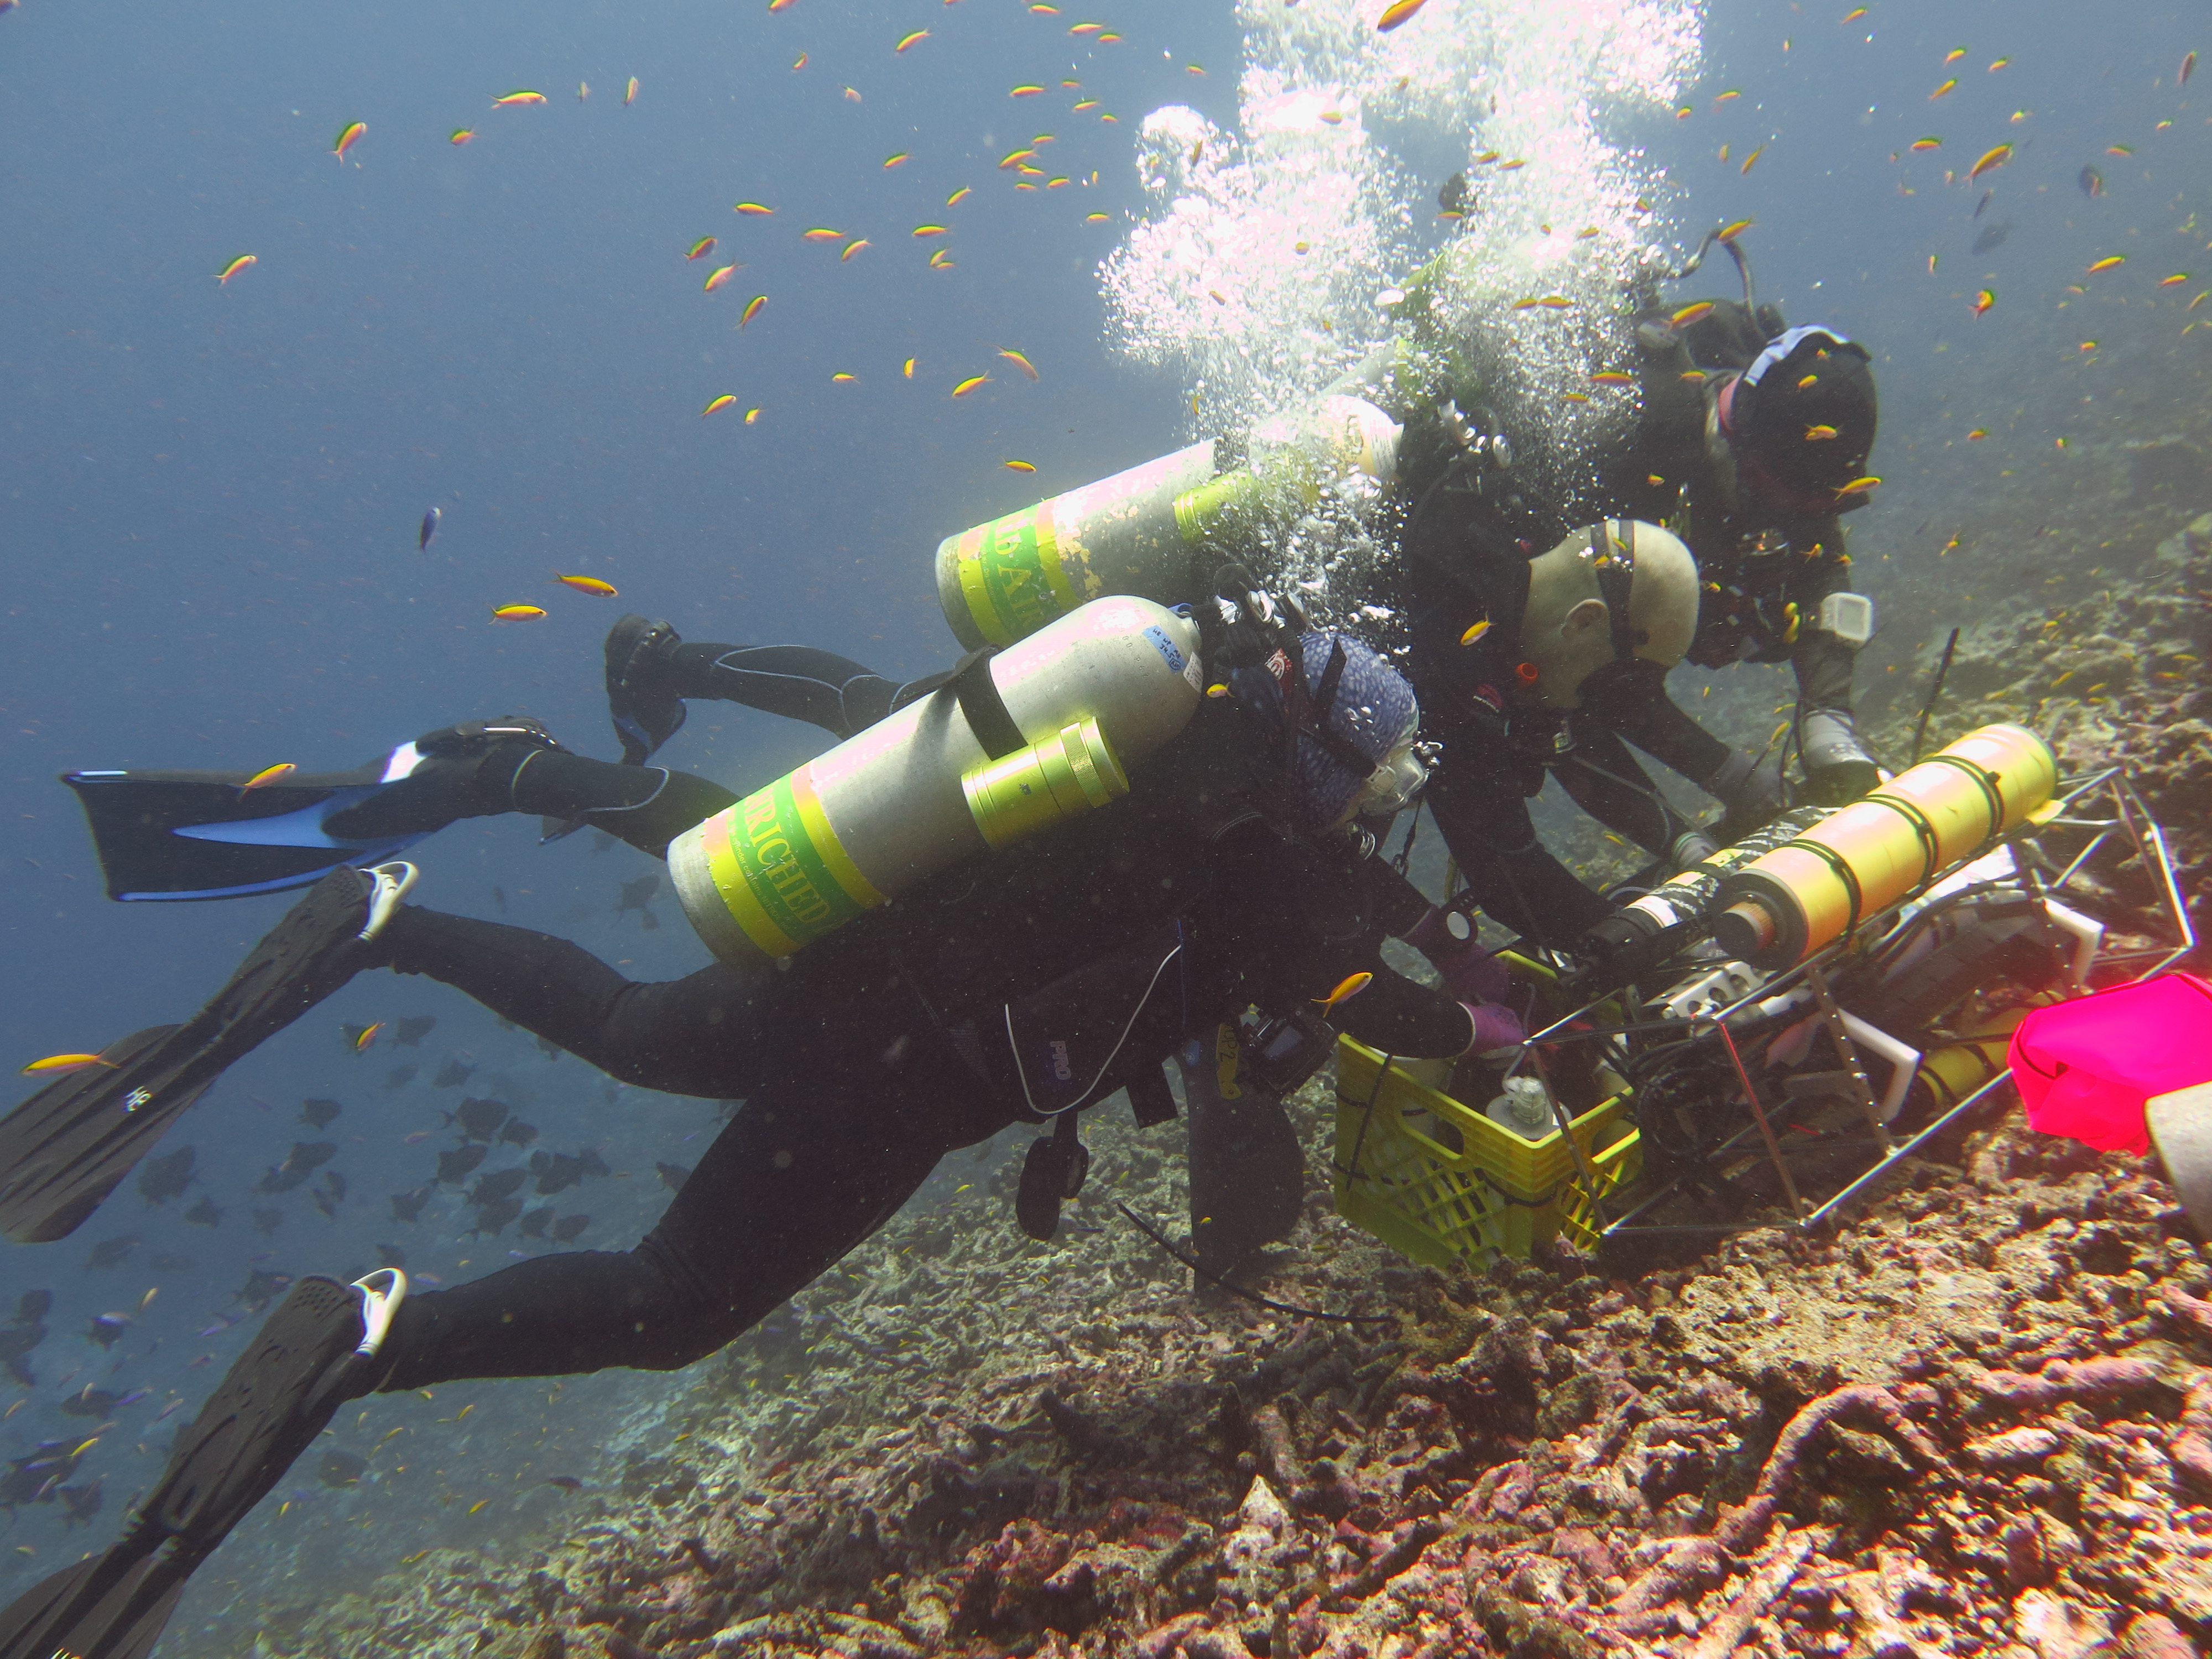
\includegraphics{images/d_suite_deploy.jpg}

\hypertarget{why-bookdown-for-the-okb}{%
\section*{Why Bookdown for the OKB?}\label{why-bookdown-for-the-okb}}
\addcontentsline{toc}{section}{Why Bookdown for the OKB?}

\hypertarget{version-control}{%
\subsection*{Version Control}\label{version-control}}
\addcontentsline{toc}{subsection}{Version Control}

we can maintain version control via github

\begin{quote}
``You've gotta get the end member.''

--- Chip Young
\end{quote}

\hypertarget{multiple-output-formats}{%
\subsection*{Multiple Output Formats}\label{multiple-output-formats}}
\addcontentsline{toc}{subsection}{Multiple Output Formats}

We can export an agile HTML version locally, a .pdf, or publish the book to R Studio Connect to be accessed via the internet.

\hypertarget{cruise_prep}{%
\chapter{Preparing for a Research Cruise}\label{cruise_prep}}

Planning for a cruise begins several months before it sails.

\hypertarget{spatial-data-preparation}{%
\section{Spatial Data Preparation}\label{spatial-data-preparation}}

\begin{itemize}
\tightlist
\item
  Create a single .kml file that includes all planned instrument retrievals and any planned additional deployments and other necessary points (collectively all called ``planning points''. .kml files are more agile than ArcGIS files; they are easier to use in Google Earth for day to day planning.
\item
  Create an ArcGIS map project that contains the locations of all planning points.
\end{itemize}

\hypertarget{garmin-78-handheld-gps-preparation}{%
\section{Garmin 78 Handheld GPS Preparation}\label{garmin-78-handheld-gps-preparation}}

\begin{itemize}
\tightlist
\item
  Ensure each handheld unit is setup properly

  \begin{itemize}
  \tightlist
  \item
    Time to UTC
  \item
    LAT and LONG in decimal degrees
  \end{itemize}
\item
  Test each handheld GPS to be taken on the cruise prior to sailing: take it outside and ensure that it collects waypoints.
\item
  Upload planning points to both the primary and secondary GPS units.
\end{itemize}

\hypertarget{datasheet-preparation}{%
\section{Datasheet Preparation}\label{datasheet-preparation}}

\begin{itemize}
\tightlist
\item
  Prepare Field Data Binders

  \begin{itemize}
  \tightlist
  \item
    Print enough data sheets for all activities, including mooring, CAU, CTD/H2O for the OCC team in addition to enough CTD/H20 data sheets for any other team on CTD/H20 Ops.
  \item
    Attach sharp pencils to field binders
  \end{itemize}
\end{itemize}

\hypertarget{software-needed-at-sea}{%
\section{Software Needed at Sea}\label{software-needed-at-sea}}

\begin{longtable}[]{@{}llllll@{}}
\toprule
\begin{minipage}[b]{0.14\columnwidth}\raggedright
Software\strut
\end{minipage} & \begin{minipage}[b]{0.06\columnwidth}\raggedright
Team Lead Only\strut
\end{minipage} & \begin{minipage}[b]{0.07\columnwidth}\raggedright
Manufacturer\strut
\end{minipage} & \begin{minipage}[b]{0.18\columnwidth}\raggedright
Needed For\strut
\end{minipage} & \begin{minipage}[b]{0.08\columnwidth}\raggedright
Instrument\strut
\end{minipage} & \begin{minipage}[b]{0.30\columnwidth}\raggedright
Download Location\strut
\end{minipage}\tabularnewline
\midrule
\endhead
\begin{minipage}[t]{0.14\columnwidth}\raggedright
ARCMap\strut
\end{minipage} & \begin{minipage}[t]{0.06\columnwidth}\raggedright
x\strut
\end{minipage} & \begin{minipage}[t]{0.07\columnwidth}\raggedright
ESRI\strut
\end{minipage} & \begin{minipage}[t]{0.18\columnwidth}\raggedright
planning operations and generating maps\strut
\end{minipage} & \begin{minipage}[t]{0.08\columnwidth}\raggedright
NA\strut
\end{minipage} & \begin{minipage}[t]{0.30\columnwidth}\raggedright
see Tomoko\strut
\end{minipage}\tabularnewline
\begin{minipage}[t]{0.14\columnwidth}\raggedright
Google Earth\strut
\end{minipage} & \begin{minipage}[t]{0.06\columnwidth}\raggedright
\strut
\end{minipage} & \begin{minipage}[t]{0.07\columnwidth}\raggedright
Google\strut
\end{minipage} & \begin{minipage}[t]{0.18\columnwidth}\raggedright
planning operations\strut
\end{minipage} & \begin{minipage}[t]{0.08\columnwidth}\raggedright
NA\strut
\end{minipage} & \begin{minipage}[t]{0.30\columnwidth}\raggedright
\strut
\end{minipage}\tabularnewline
\begin{minipage}[t]{0.14\columnwidth}\raggedright
Keyspan USA Software\strut
\end{minipage} & \begin{minipage}[t]{0.06\columnwidth}\raggedright
\strut
\end{minipage} & \begin{minipage}[t]{0.07\columnwidth}\raggedright
Keyspan\strut
\end{minipage} & \begin{minipage}[t]{0.18\columnwidth}\raggedright
serial to USB adapter cable\strut
\end{minipage} & \begin{minipage}[t]{0.08\columnwidth}\raggedright
GPS\strut
\end{minipage} & \begin{minipage}[t]{0.30\columnwidth}\raggedright
\url{https://www.tripplite.com/support/USA19HS}\strut
\end{minipage}\tabularnewline
\begin{minipage}[t]{0.14\columnwidth}\raggedright
Microsoft Access 2010\strut
\end{minipage} & \begin{minipage}[t]{0.06\columnwidth}\raggedright
\strut
\end{minipage} & \begin{minipage}[t]{0.07\columnwidth}\raggedright
Microsoft\strut
\end{minipage} & \begin{minipage}[t]{0.18\columnwidth}\raggedright
mooring and CTD databases\strut
\end{minipage} & \begin{minipage}[t]{0.08\columnwidth}\raggedright
NA\strut
\end{minipage} & \begin{minipage}[t]{0.30\columnwidth}\raggedright
request from ITS\strut
\end{minipage}\tabularnewline
\begin{minipage}[t]{0.14\columnwidth}\raggedright
Excel\strut
\end{minipage} & \begin{minipage}[t]{0.06\columnwidth}\raggedright
\strut
\end{minipage} & \begin{minipage}[t]{0.07\columnwidth}\raggedright
Microsoft\strut
\end{minipage} & \begin{minipage}[t]{0.18\columnwidth}\raggedright
spreadsheets\strut
\end{minipage} & \begin{minipage}[t]{0.08\columnwidth}\raggedright
NA\strut
\end{minipage} & \begin{minipage}[t]{0.30\columnwidth}\raggedright
you must have this already\strut
\end{minipage}\tabularnewline
\begin{minipage}[t]{0.14\columnwidth}\raggedright
DNR Garmin\strut
\end{minipage} & \begin{minipage}[t]{0.06\columnwidth}\raggedright
\strut
\end{minipage} & \begin{minipage}[t]{0.07\columnwidth}\raggedright
Minnesota DNR\strut
\end{minipage} & \begin{minipage}[t]{0.18\columnwidth}\raggedright
download of GPS Waypoints\strut
\end{minipage} & \begin{minipage}[t]{0.08\columnwidth}\raggedright
GPS\strut
\end{minipage} & \begin{minipage}[t]{0.30\columnwidth}\raggedright
\url{http://www.dnr.state.mn.us/mis/gis/tools/arcview/extensions/DNRGarmin/DNRGarmin.html}\strut
\end{minipage}\tabularnewline
\begin{minipage}[t]{0.14\columnwidth}\raggedright
DNR GPS\strut
\end{minipage} & \begin{minipage}[t]{0.06\columnwidth}\raggedright
\strut
\end{minipage} & \begin{minipage}[t]{0.07\columnwidth}\raggedright
Minnesota DNR\strut
\end{minipage} & \begin{minipage}[t]{0.18\columnwidth}\raggedright
upload of GPS planning points from Google Earth\strut
\end{minipage} & \begin{minipage}[t]{0.08\columnwidth}\raggedright
GPS\strut
\end{minipage} & \begin{minipage}[t]{0.30\columnwidth}\raggedright
\url{http://www.dnr.state.mn.us/mis/gis/DNRGPS/DNRGPS.html}\strut
\end{minipage}\tabularnewline
\begin{minipage}[t]{0.14\columnwidth}\raggedright
Aquadopp Software - AquaPro v1.37.08\strut
\end{minipage} & \begin{minipage}[t]{0.06\columnwidth}\raggedright
\strut
\end{minipage} & \begin{minipage}[t]{0.07\columnwidth}\raggedright
Nortek\strut
\end{minipage} & \begin{minipage}[t]{0.18\columnwidth}\raggedright
instrument interface\strut
\end{minipage} & \begin{minipage}[t]{0.08\columnwidth}\raggedright
Aquadopp ADCP\strut
\end{minipage} & \begin{minipage}[t]{0.30\columnwidth}\raggedright
\url{http://www.nortek-as.com/en/support/software}\strut
\end{minipage}\tabularnewline
\begin{minipage}[t]{0.14\columnwidth}\raggedright
SoundTrap Host Software Version 2.0.9.x\strut
\end{minipage} & \begin{minipage}[t]{0.06\columnwidth}\raggedright
x\strut
\end{minipage} & \begin{minipage}[t]{0.07\columnwidth}\raggedright
Ocean Instruments\strut
\end{minipage} & \begin{minipage}[t]{0.18\columnwidth}\raggedright
instrument interface\strut
\end{minipage} & \begin{minipage}[t]{0.08\columnwidth}\raggedright
Sound Trap\strut
\end{minipage} & \begin{minipage}[t]{0.30\columnwidth}\raggedright
\url{http://www.oceaninstruments.co.nz/downloads/}\strut
\end{minipage}\tabularnewline
\begin{minipage}[t]{0.14\columnwidth}\raggedright
Basic Stamp Editor\strut
\end{minipage} & \begin{minipage}[t]{0.06\columnwidth}\raggedright
\strut
\end{minipage} & \begin{minipage}[t]{0.07\columnwidth}\raggedright
Paralax Inc.\strut
\end{minipage} & \begin{minipage}[t]{0.18\columnwidth}\raggedright
instrument interface\strut
\end{minipage} & \begin{minipage}[t]{0.08\columnwidth}\raggedright
PUC\strut
\end{minipage} & \begin{minipage}[t]{0.30\columnwidth}\raggedright
\url{https://www.parallax.com/downloads/basic-stamp-editor-software-windows}\strut
\end{minipage}\tabularnewline
\begin{minipage}[t]{0.14\columnwidth}\raggedright
Python 2.51\strut
\end{minipage} & \begin{minipage}[t]{0.06\columnwidth}\raggedright
\strut
\end{minipage} & \begin{minipage}[t]{0.07\columnwidth}\raggedright
Python\strut
\end{minipage} & \begin{minipage}[t]{0.18\columnwidth}\raggedright
scripts that are part of mooring and CTD databases\strut
\end{minipage} & \begin{minipage}[t]{0.08\columnwidth}\raggedright
NA\strut
\end{minipage} & \begin{minipage}[t]{0.30\columnwidth}\raggedright
\url{https://www.python.org/download/releases/2.5.1/}\strut
\end{minipage}\tabularnewline
\begin{minipage}[t]{0.14\columnwidth}\raggedright
SeaFETCOM 2\strut
\end{minipage} & \begin{minipage}[t]{0.06\columnwidth}\raggedright
\strut
\end{minipage} & \begin{minipage}[t]{0.07\columnwidth}\raggedright
Satlantic\strut
\end{minipage} & \begin{minipage}[t]{0.18\columnwidth}\raggedright
instrument interface\strut
\end{minipage} & \begin{minipage}[t]{0.08\columnwidth}\raggedright
SeaFet\strut
\end{minipage} & \begin{minipage}[t]{0.30\columnwidth}\raggedright
\url{http://satlantic.com/seafetcom}\strut
\end{minipage}\tabularnewline
\begin{minipage}[t]{0.14\columnwidth}\raggedright
Seaterm 1.59\strut
\end{minipage} & \begin{minipage}[t]{0.06\columnwidth}\raggedright
\strut
\end{minipage} & \begin{minipage}[t]{0.07\columnwidth}\raggedright
SeaBird\strut
\end{minipage} & \begin{minipage}[t]{0.18\columnwidth}\raggedright
instrument interface\strut
\end{minipage} & \begin{minipage}[t]{0.08\columnwidth}\raggedright
SBE39, SBE19, SBE19+\strut
\end{minipage} & \begin{minipage}[t]{0.30\columnwidth}\raggedright
\url{http://www.seabird.com/software/software}\strut
\end{minipage}\tabularnewline
\begin{minipage}[t]{0.14\columnwidth}\raggedright
Seaterm V2\strut
\end{minipage} & \begin{minipage}[t]{0.06\columnwidth}\raggedright
\strut
\end{minipage} & \begin{minipage}[t]{0.07\columnwidth}\raggedright
SeaBird\strut
\end{minipage} & \begin{minipage}[t]{0.18\columnwidth}\raggedright
instrument interface\strut
\end{minipage} & \begin{minipage}[t]{0.08\columnwidth}\raggedright
sbe19+ V2, SBE56\strut
\end{minipage} & \begin{minipage}[t]{0.30\columnwidth}\raggedright
\url{http://www.seabird.com/software/software}\strut
\end{minipage}\tabularnewline
\begin{minipage}[t]{0.14\columnwidth}\raggedright
SBE Data Processing\strut
\end{minipage} & \begin{minipage}[t]{0.06\columnwidth}\raggedright
\strut
\end{minipage} & \begin{minipage}[t]{0.07\columnwidth}\raggedright
SeaBird\strut
\end{minipage} & \begin{minipage}[t]{0.18\columnwidth}\raggedright
CTD cast processing\strut
\end{minipage} & \begin{minipage}[t]{0.08\columnwidth}\raggedright
SBE CTDs\strut
\end{minipage} & \begin{minipage}[t]{0.30\columnwidth}\raggedright
\url{https://www.seabird.com/software-updates}\strut
\end{minipage}\tabularnewline
\begin{minipage}[t]{0.14\columnwidth}\raggedright
R and R Studio for STR processing\strut
\end{minipage} & \begin{minipage}[t]{0.06\columnwidth}\raggedright
\strut
\end{minipage} & \begin{minipage}[t]{0.07\columnwidth}\raggedright
R Studio\strut
\end{minipage} & \begin{minipage}[t]{0.18\columnwidth}\raggedright
data processing\strut
\end{minipage} & \begin{minipage}[t]{0.08\columnwidth}\raggedright
all\strut
\end{minipage} & \begin{minipage}[t]{0.30\columnwidth}\raggedright
\url{https://www.rstudio.com/products/rstudio/download/}\strut
\end{minipage}\tabularnewline
\begin{minipage}[t]{0.14\columnwidth}\raggedright
Ruskin\strut
\end{minipage} & \begin{minipage}[t]{0.06\columnwidth}\raggedright
\strut
\end{minipage} & \begin{minipage}[t]{0.07\columnwidth}\raggedright
RBR\strut
\end{minipage} & \begin{minipage}[t]{0.18\columnwidth}\raggedright
STR, PAR, DO\strut
\end{minipage} & \begin{minipage}[t]{0.08\columnwidth}\raggedright
RBR Solo\strut
\end{minipage} & \begin{minipage}[t]{0.30\columnwidth}\raggedright
\url{https://rbr-global.com/products/software}\strut
\end{minipage}\tabularnewline
\bottomrule
\end{longtable}

\hypertarget{ctd-and-dic-water-sampling}{%
\chapter{CTD and DIC Water Sampling}\label{ctd-and-dic-water-sampling}}

If available hands on deck and conditions allow, please conduct the CTD downcast and the water sample collection simultaneously.

\hypertarget{waypoint-and-metadata-collection}{%
\section{Waypoint and metadata collection}\label{waypoint-and-metadata-collection}}

Use the OCC provided GPS unit to collect a waypoint when the CTD downcast begins. Record all metadata on provided data sheet.

\hypertarget{ctd-cast}{%
\section{CTD CAST}\label{ctd-cast}}

\begin{enumerate}
\def\labelenumi{\arabic{enumi}.}
\tightlist
\item
  Ensure that the CTD line is connected to the top of the CTD frame by 1 shackles.
\item
  Tie non-CTD end of the CTD line to the boat with a bowline or clip off with carabiner.
\item
  Flake CTD line on deck.
\item
  When the coxswain says the CTD can go over the side, raise the CTD switch to the ``ON'' position, and loudly say, ``ON!'' then lower it over the side until the top of the frame is 1 meter below the surface of the water to begin the 1 minute soaking period, either holding the line or cleating off the line to maintain the CTD at soaking depth.
\item
  After 1 minute soak, ask the coxswain for the current depth so you know how far you can lower the CTD without it hitting the bottom (5-10 feet less line than the bottom depth). Un-cleat the CTD line if it was cleated and begin the CTD cast by pulling the CTD frame up until the top ring of the frame emerges from the water, then begin gradually lowering at a consistent rate, hand over hand, until the CTD gets to the target depth (using the markings on the line to estimate depth). Once the target depth is reached, pull the CTD back on board.
\item
  Once the CTD is back on board, lower the switch to ``OFF'', and loudly say ``OFF!''
\end{enumerate}

\hypertarget{water-sample-collection}{%
\section{water sample collection}\label{water-sample-collection}}

\begin{enumerate}
\def\labelenumi{\arabic{enumi}.}
\tightlist
\item
  Prime the Niskin Bottle, ensuring the petcock and the air bleed valve are closed.
\item
  Clip off the boat side of the niskin line to the boat.
\item
  Near the end of the the CTD soaking time, lower the weight and the open Niskin bottle over the side so the top of the Niskin is at 1m depth (surface of water at the BLACK mark drawn on Niskin line).
\item
  Clip the messenger on to the line
\item
  When the CTD begins its downcast, send the messenger to trigger the Niskin to close. Ensure no air bubbles are trapped inside the Niskin and bottle sits vertically in the water column before firing the messenger.
\end{enumerate}

\hypertarget{water-sample-processing}{%
\section{Water sample Processing}\label{water-sample-processing}}

\begin{enumerate}
\def\labelenumi{\arabic{enumi}.}
\item
  Designate roles: bottle filler, mercuric chloride (HgCl2) handler, data recorder. NOTE: Supersaturated mercuric chloride solution is extremely dangerous; use the utmost caution when dealing with the chemical. All personnel working with it are required to wear eye protection. The mercuric chloride handler is also required to where disposable nitrile gloves. In the event of contact with any part of the body, wash the area profusely. If contact is made with eyes, abort operations, rinse continuously with fresh water (or salt if fresh has run out), alert the ship and return ASAP.
\item
  Remove a bottle and its stopper from the storage tote and insert the tygon tubing to the bottom of the bottle. With the tygon tubing attached to the Niskin bottle dispensing nipple, open the Niskin bottle valve and allow for three complete flushings of the bottle to occur before stopping the sample collection (i.e.~start the collection and count how long it takes for the bottle to overflow and then allow that to occur for 2x the required fill time\ldots ie. if the bottle fills in 20 seconds, allow the sample water flow to flush the bottle for 60 seconds). Attention must be given to how the sample water enters the bottle. Care should be given to ensure that smooth water flow into the bottle is maintained and that no bubbles are created during the dispensing of sample. Any bubbles introduced to the sample will alter the pCO2 within the sample water and produce inaccurate DIC results.
\item
  After the appropriate flushing time, shut off the Niskin valve to stop the water flow, while at the same time ensuring the tygon tubing doesn't come off the bottom of the sample bottle. Once the flow is shut off, pinch the tubing and in one motion remove it from the bottle. This ``pinch and remove'' action with the tubing should establish a consistent head-space in all the sample bottles. The meniscus of the sample should be about 1 cm below the neck of the bottle (see picture.)
  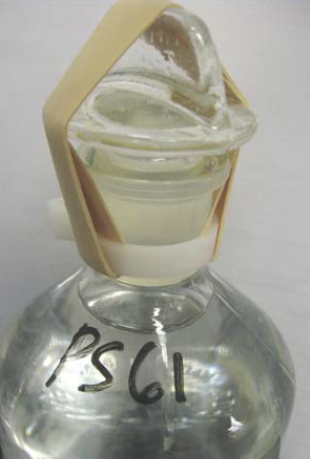
\includegraphics{images/BOD_bottle_headspace.png}
\item
  \begin{enumerate}
  \def\labelenumii{\alph{enumii}.}
  \tightlist
  \item
    Once the proper head space is established, pipette 200ul of HgCl2 saturated solution into the sample bottle
  \item
    Use the syringe containing vacuum grease to make 3-5 vertical ``stripes'' of grease on a clean, dry stopper. Insert the greased stopper until fully seated in the bottle, then twist until the grease completely seals the bottle contents. The vertical stripes of grease allow for gases to escape the bottle neck while the stopper is being inserted. Having the stopper clean/dry ensures that other than sample water isn't introduced into the bottle. Twisting the stopper, once it has been fully seated into the neck of the bottle, ensures a smooth distribution of grease within the sample bottle's neck and an air tight seal.
  \item
    Use the rubber band and plastic collar to lock down the stopper inside the bottle. Once secured, softly invert the bottle 1-2x to mix the HgCl2 with the water sampleand secure the sample bottle in the field container.
  \item
    Complete data sheet including REA Site name or OCC Site Name (if it exists), waypoint name (default), UTC date and time, lat and long, sample depth and DIC bottle \#.
  \end{enumerate}
\end{enumerate}

\hypertarget{mercuric-chloride-emergency-procedures}{%
\section{Mercuric Chloride Emergency Procedures}\label{mercuric-chloride-emergency-procedures}}

\begin{itemize}
\tightlist
\item
  Eyes: Irrigate immediately with large quantity of water for at least 15 minutes.
\item
  Skin: Immediately flush with plenty of water for at least 15 minutes. Remove any contaminated clothing.
\item
  Inhalation: Remove to fresh air. If not breathing, give artificial respiration. If breathing is difficult, give oxygen.
\item
  Ingestion: Only induce vomiting if directed to do so by medical personnel.
\item
  The MSDS can be seen from any NOAA Google Account via \href{https://drive.google.com/open?id=12w0Kmi8VVE9n_0A5_BhNVq6l4nMDtM1K}{this google drive link}
\end{itemize}

\hypertarget{mercuric-chloride-safety-data-sheet-sds}{%
\subsection{Mercuric Chloride Safety Data Sheet (SDS)}\label{mercuric-chloride-safety-data-sheet-sds}}

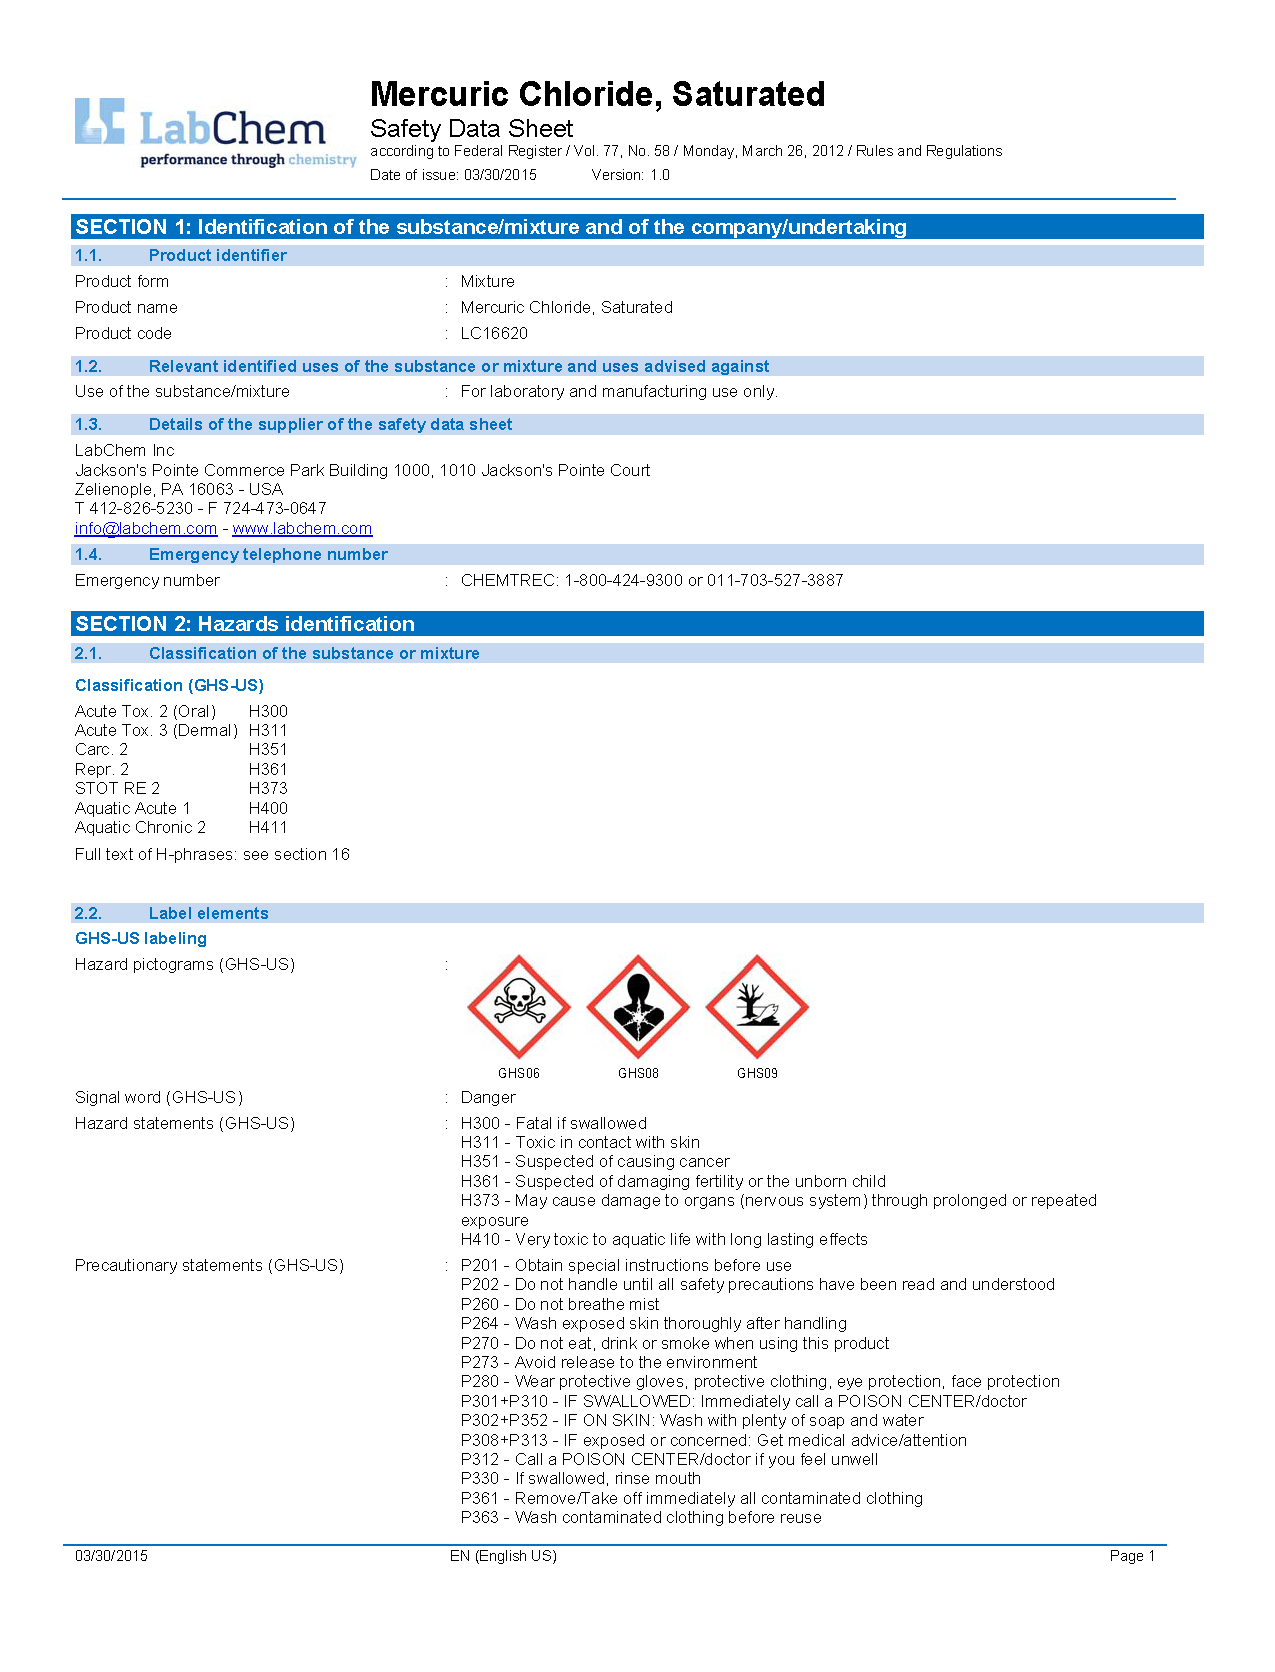
\includegraphics[width=1\textwidth,height=\textheight]{images/Saturated-Mercuric-Chloride-SDS_Page_1.png}
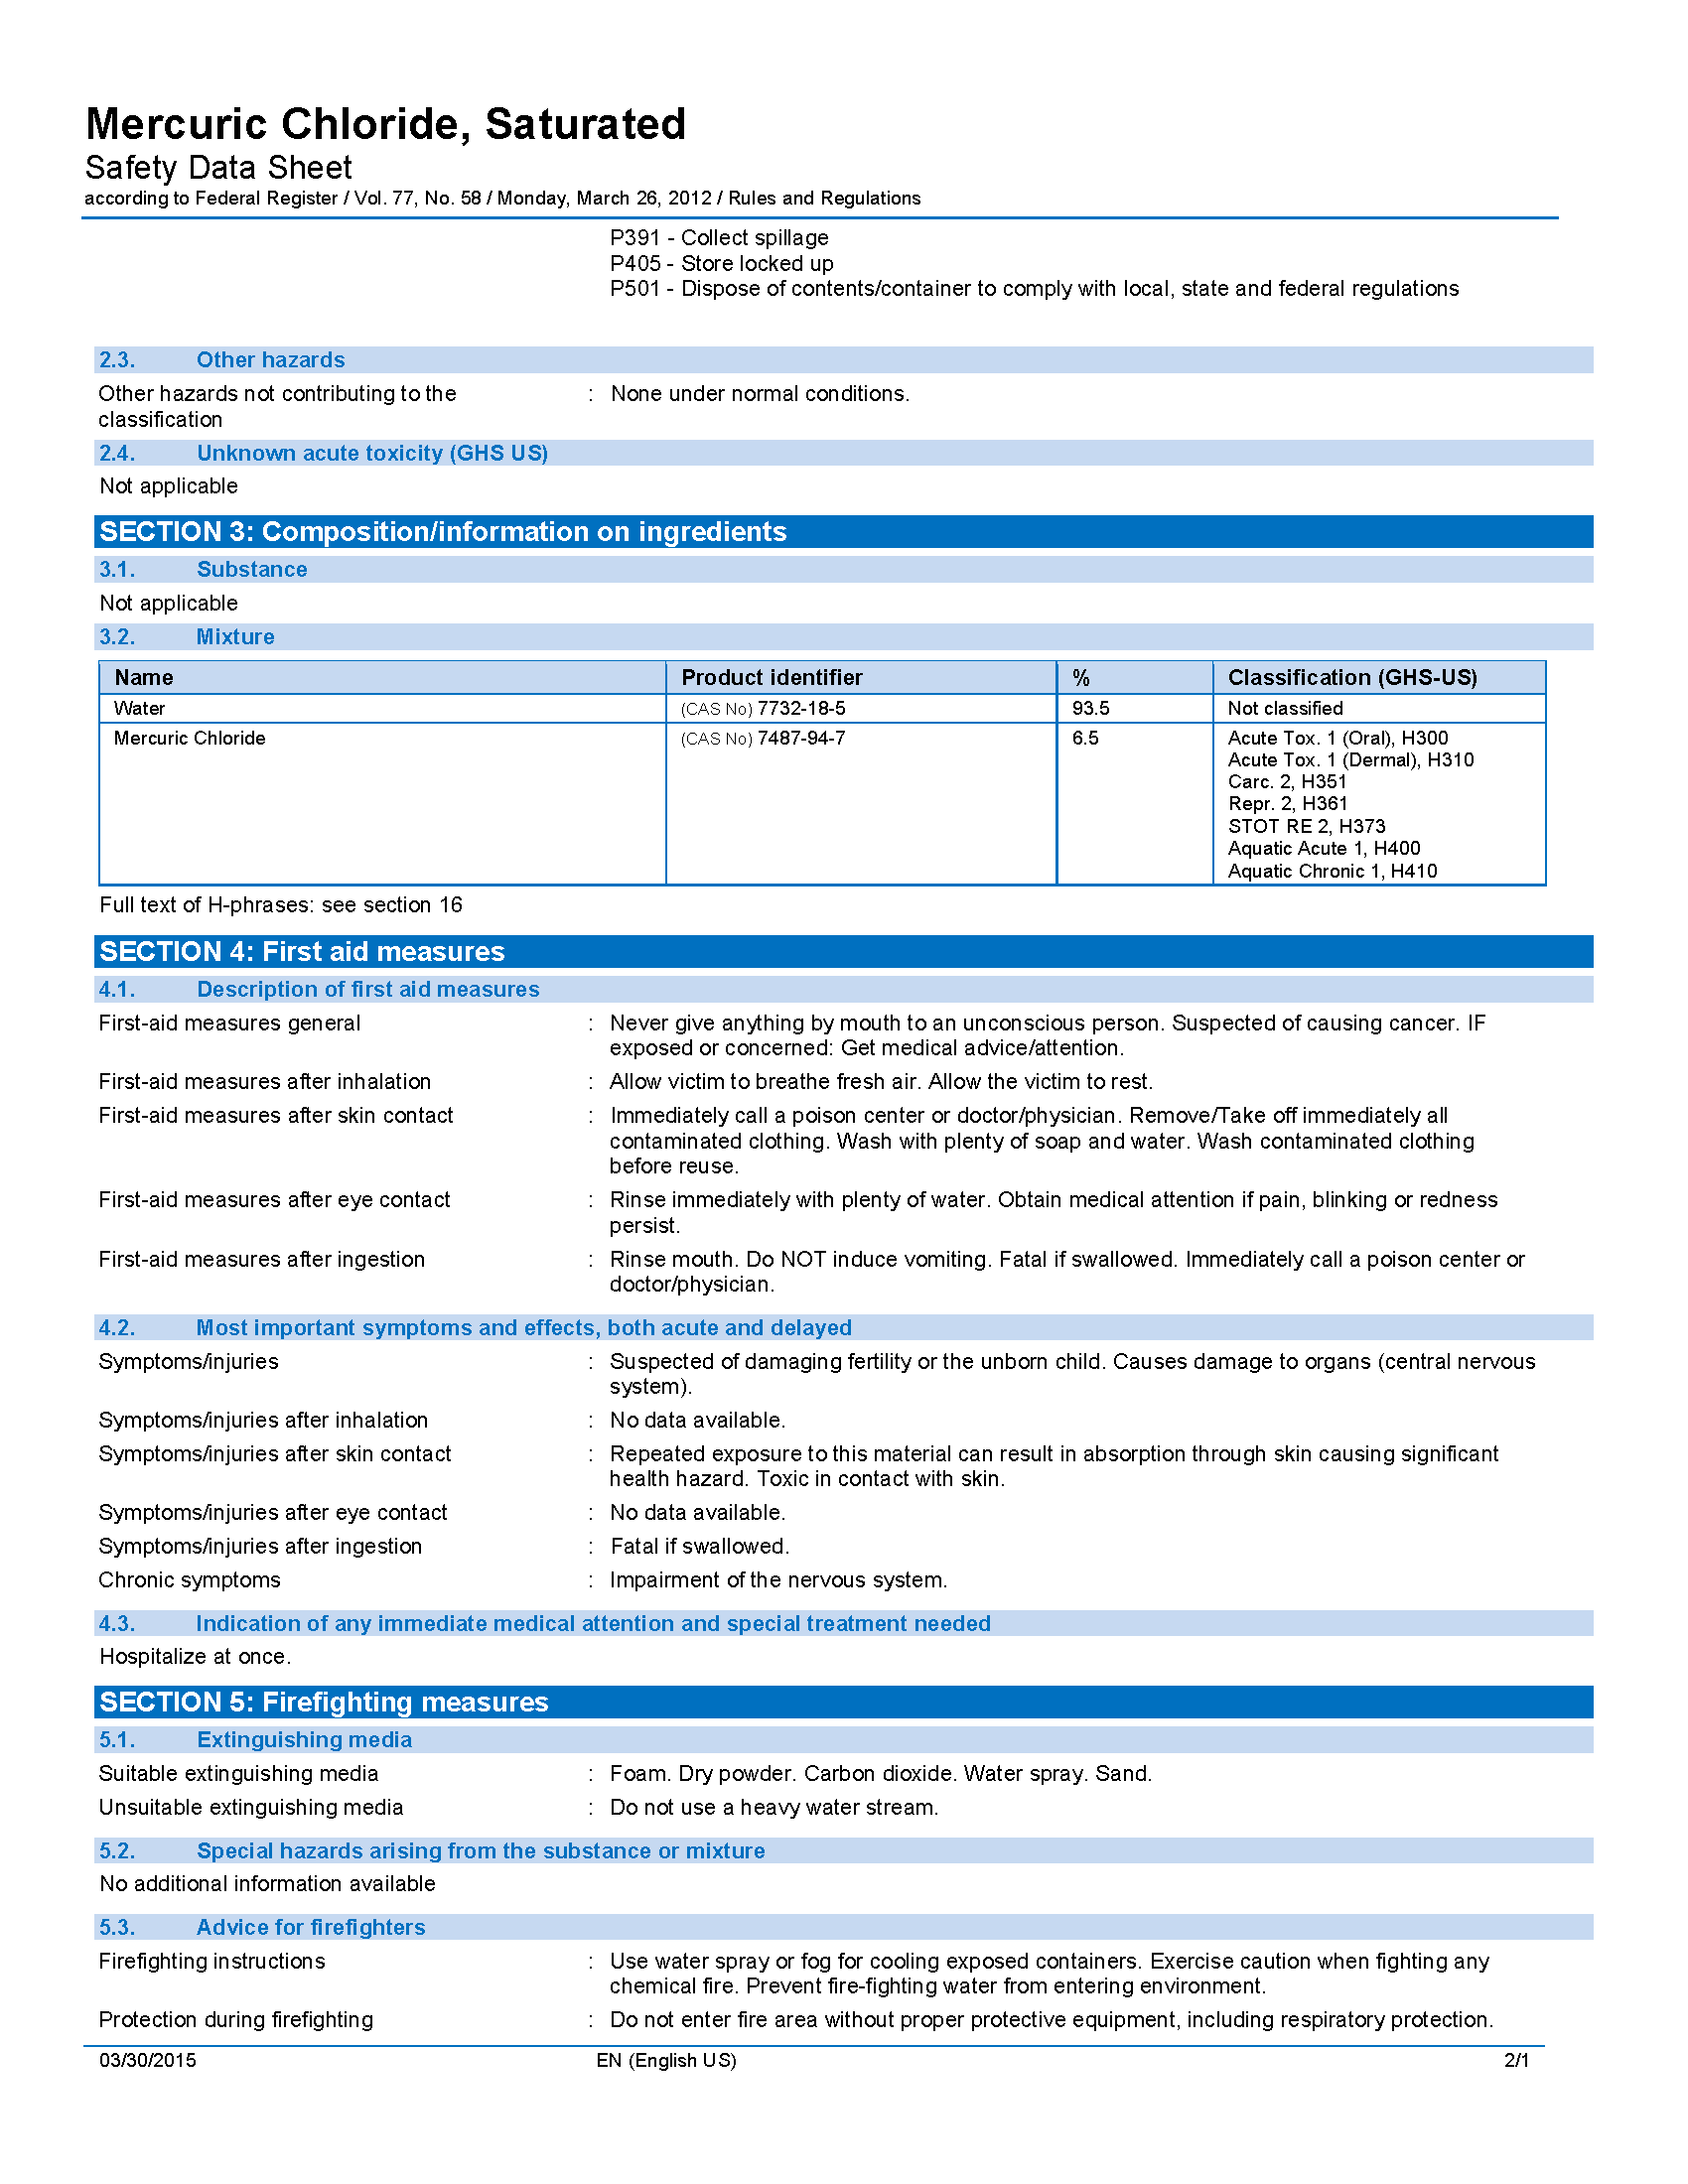
\includegraphics[width=1\textwidth,height=\textheight]{images/Saturated-Mercuric-Chloride-SDS_Page_2.png}
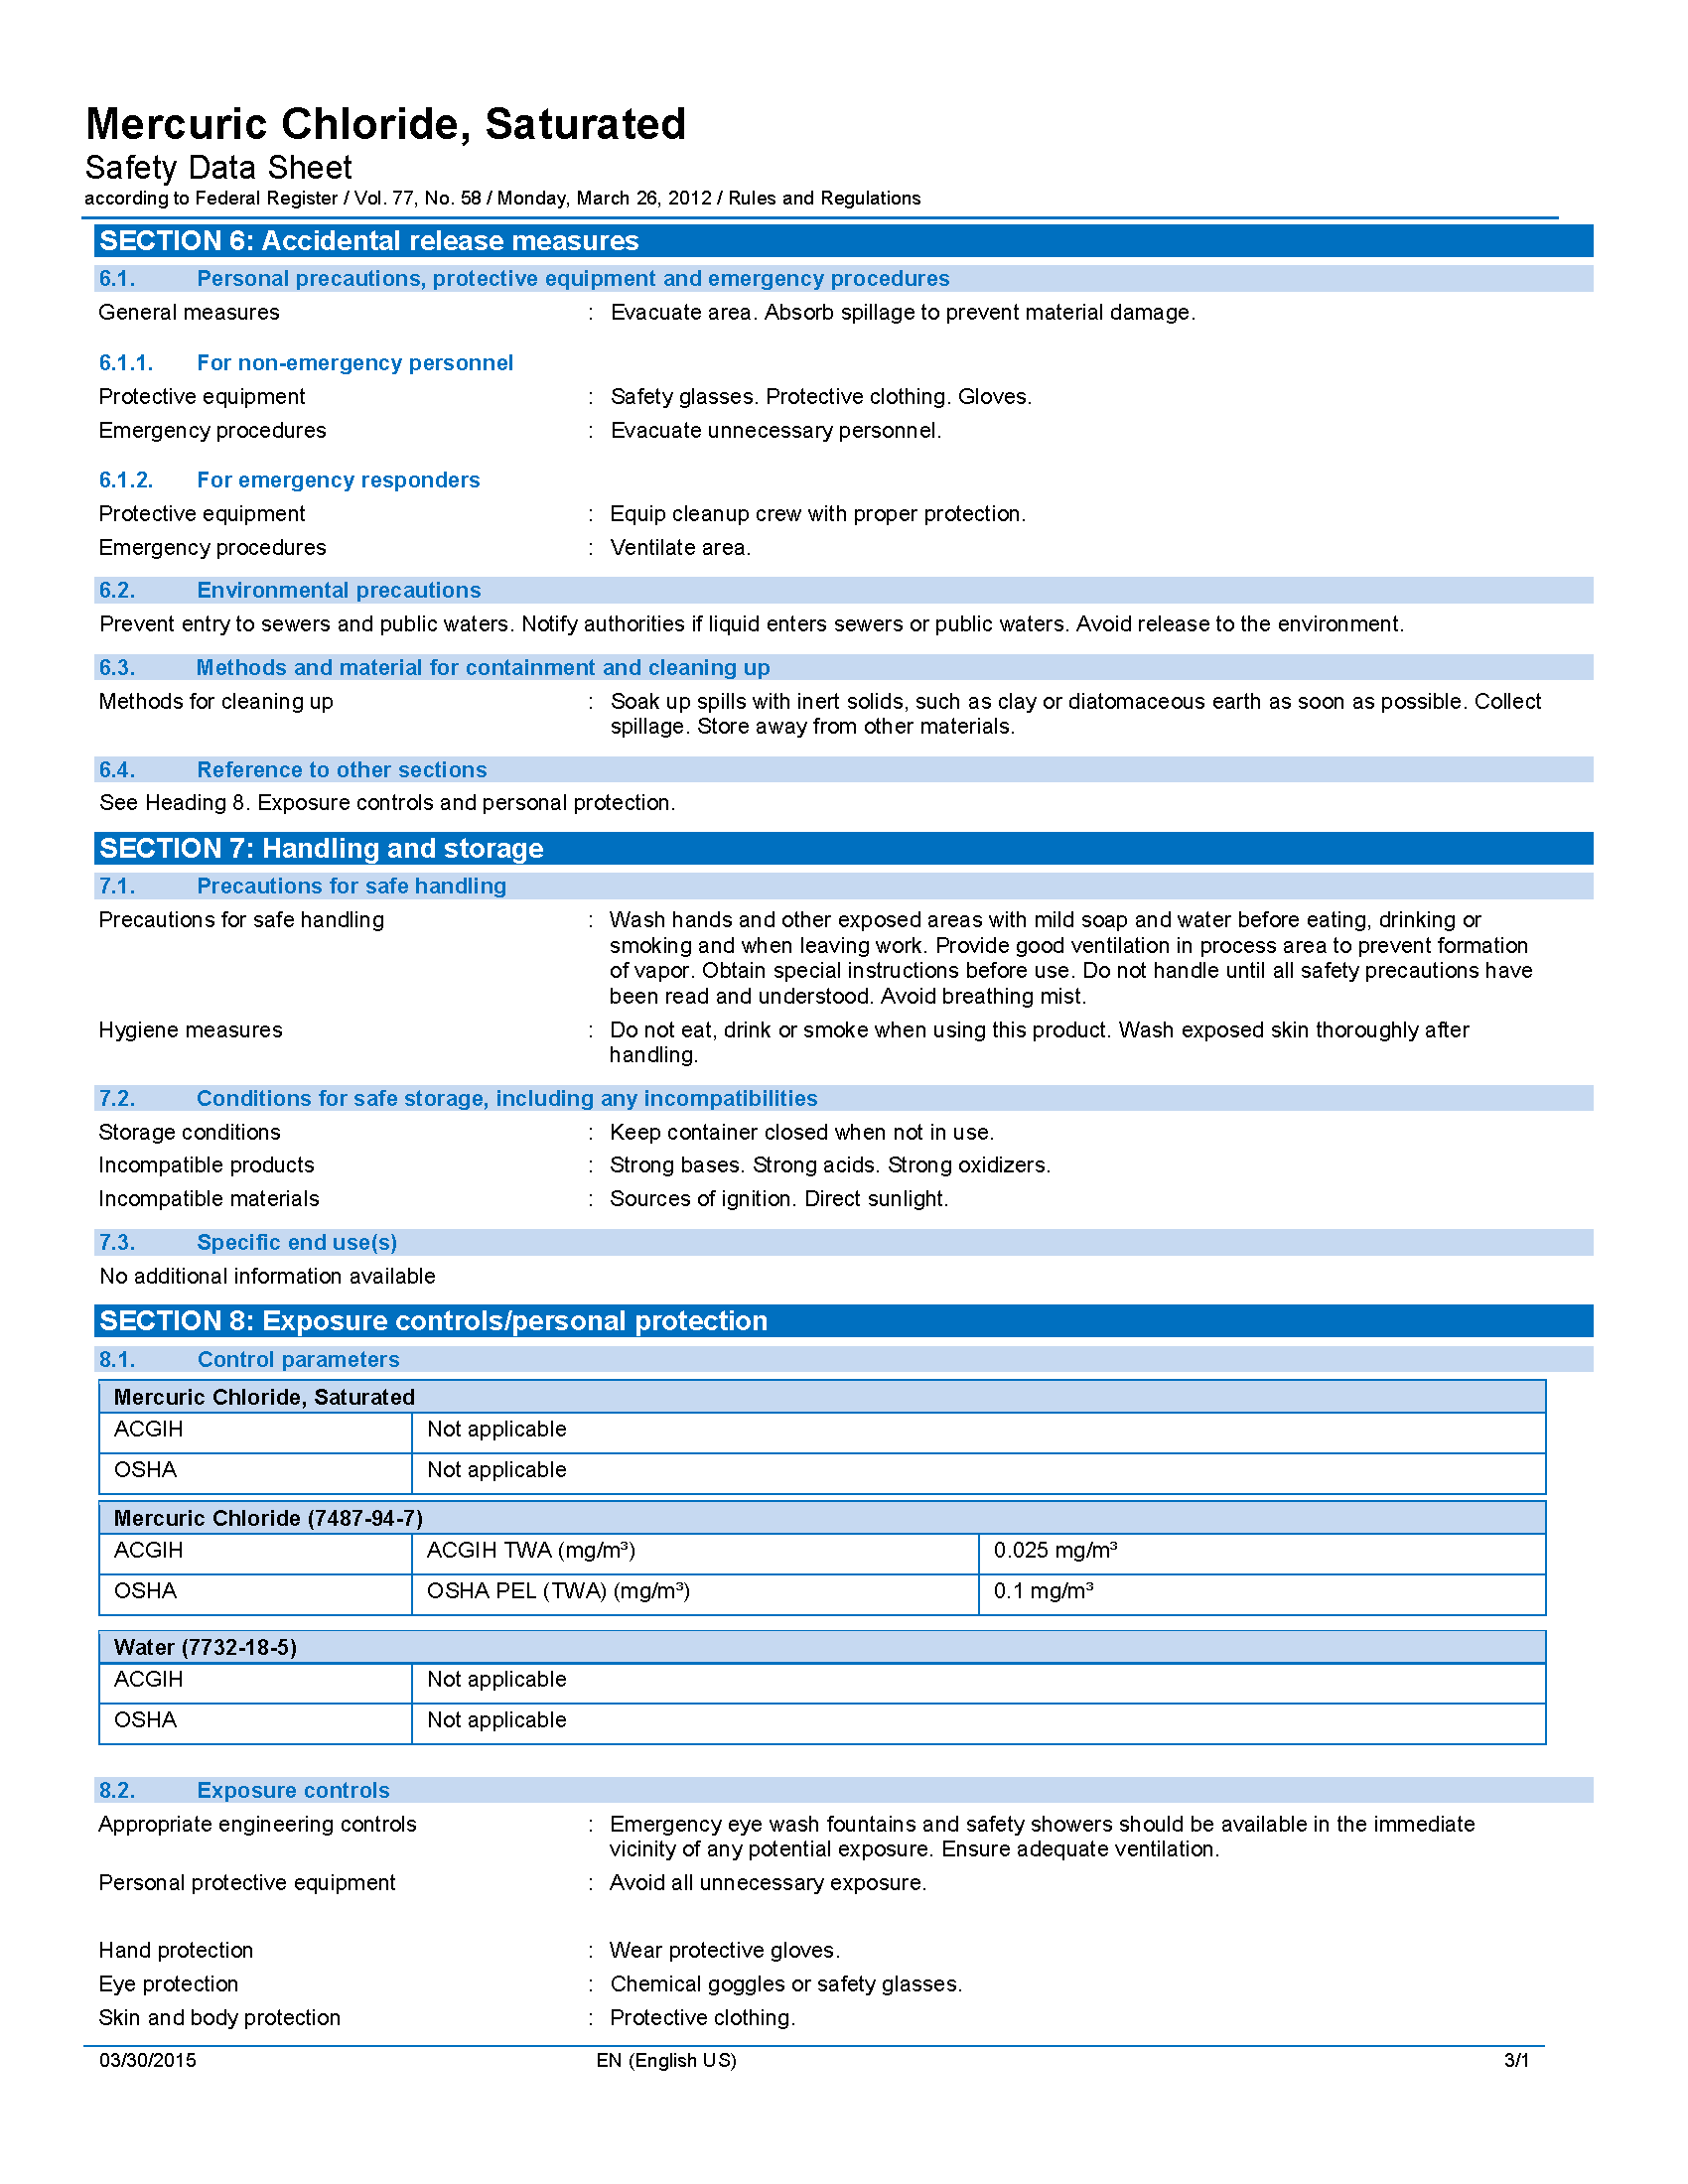
\includegraphics[width=1\textwidth,height=\textheight]{images/Saturated-Mercuric-Chloride-SDS_Page_3.png}
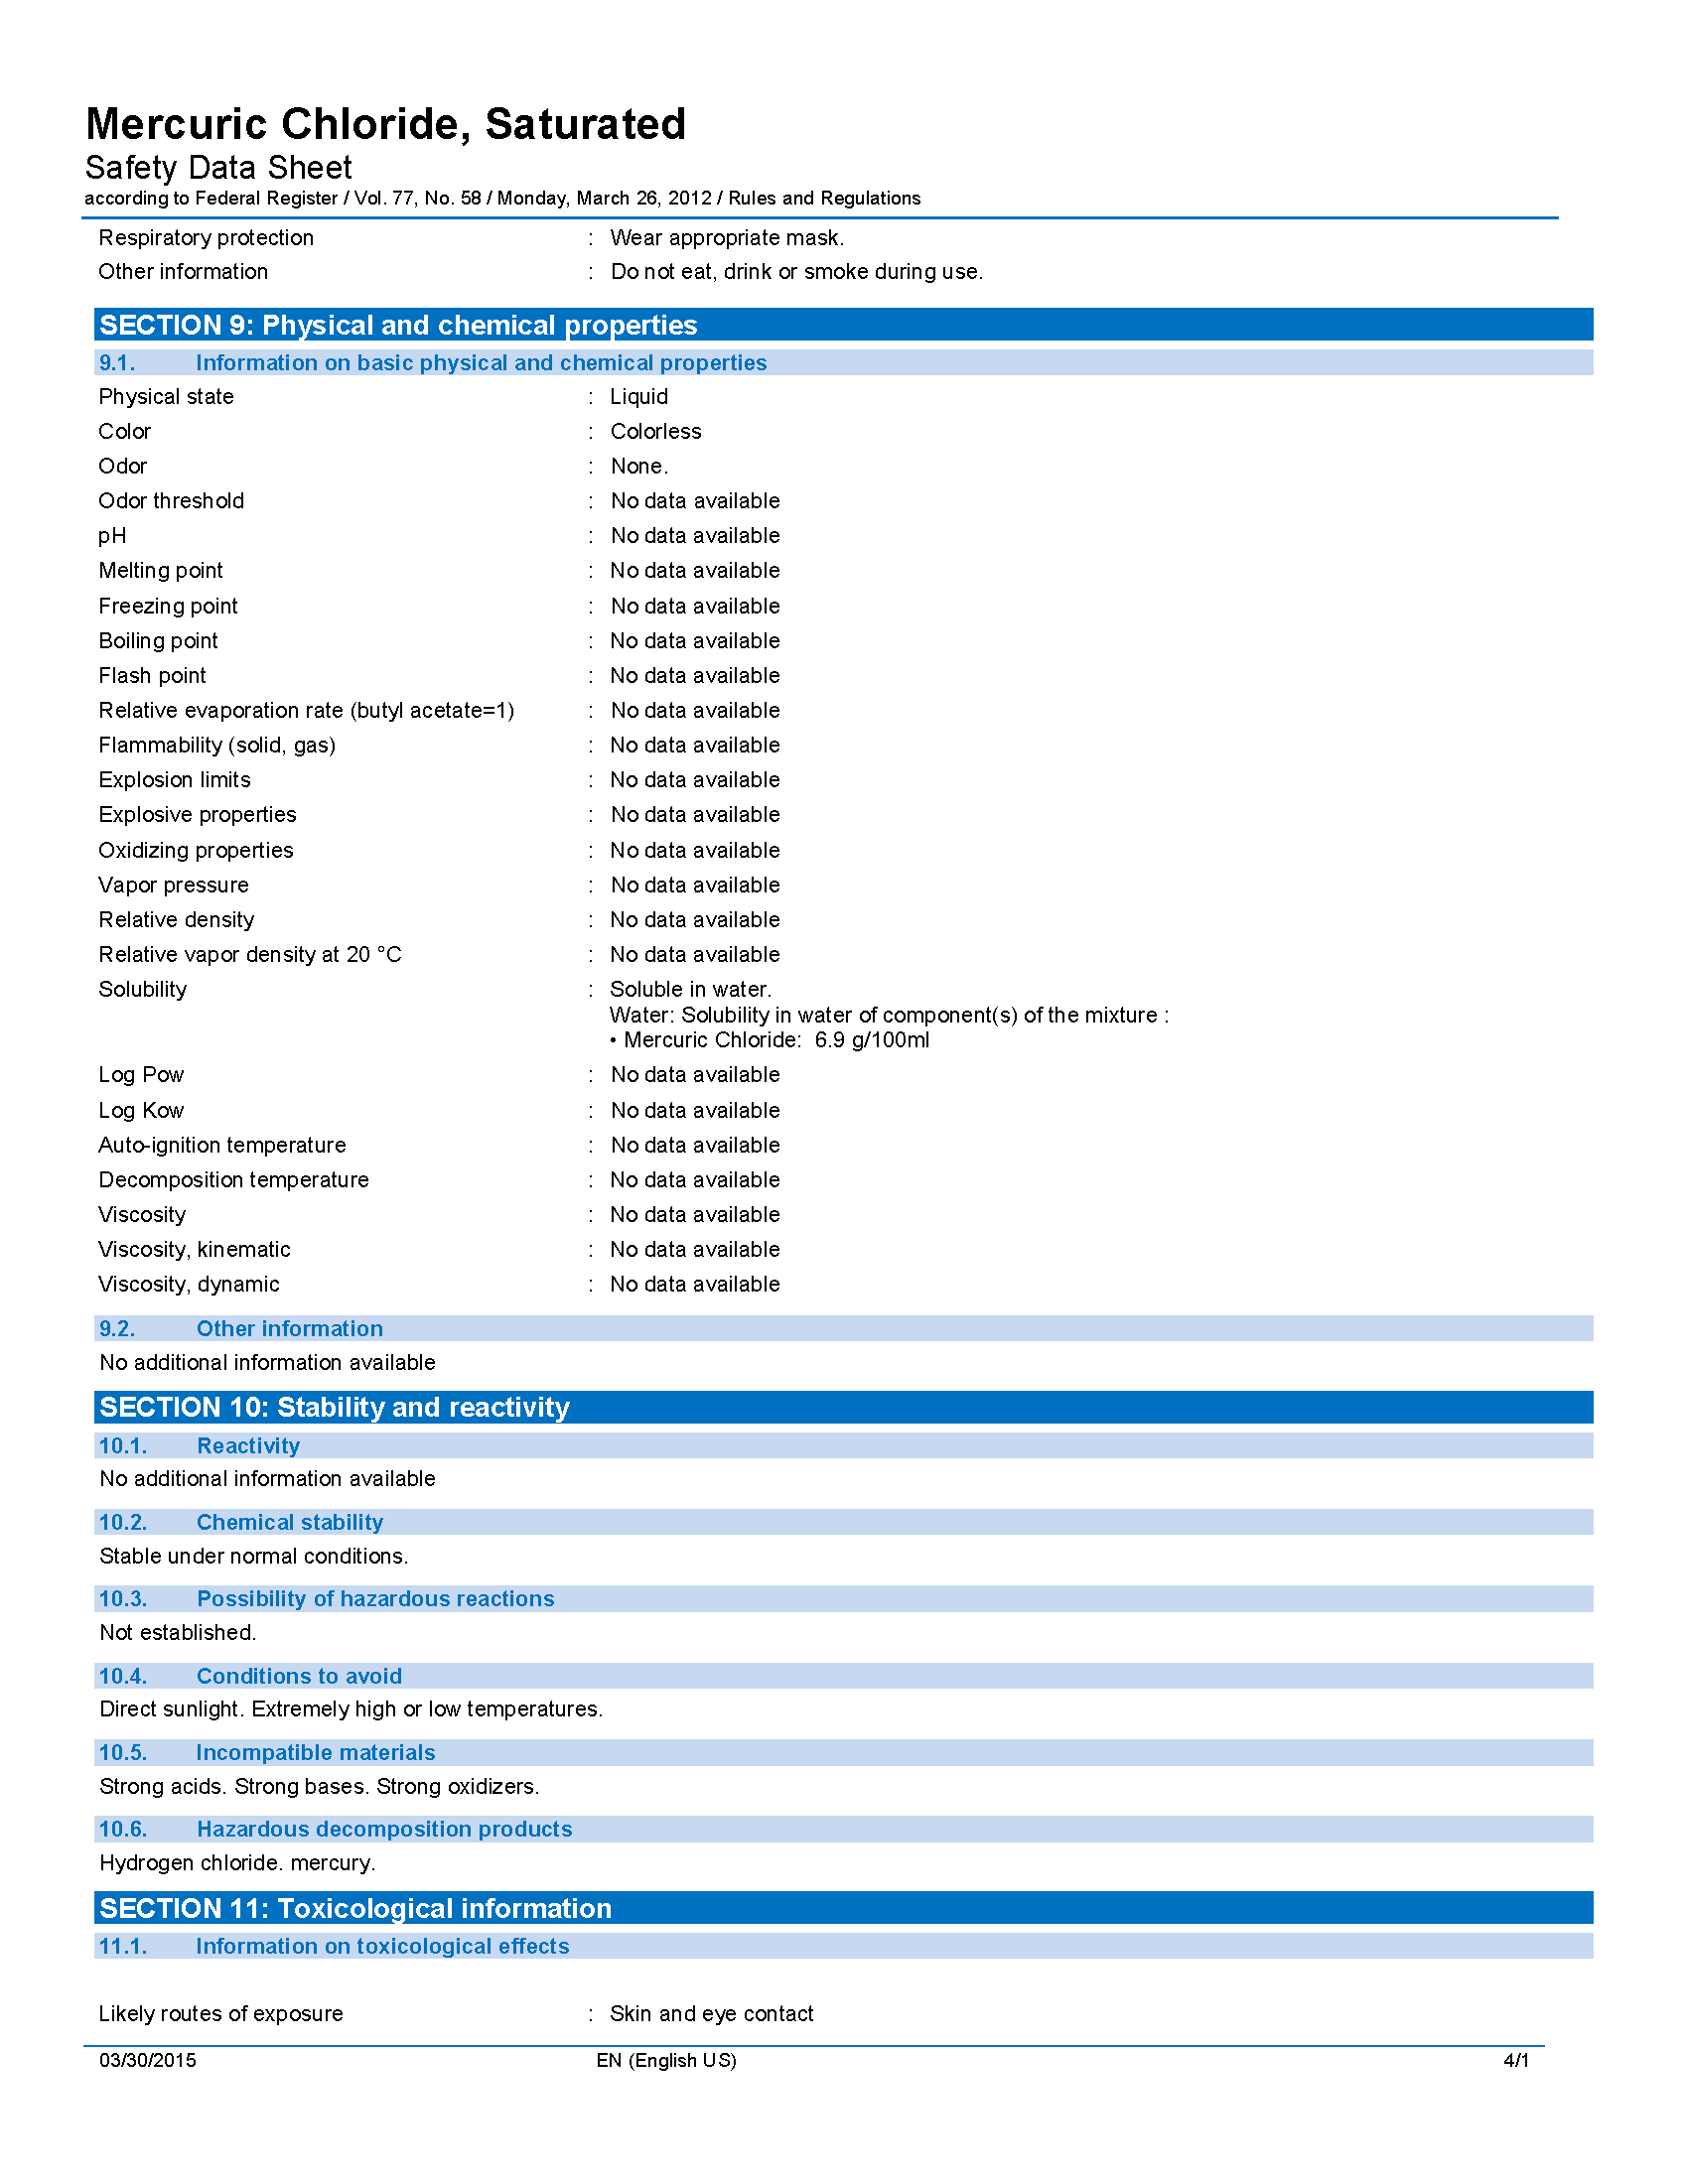
\includegraphics[width=1\textwidth,height=\textheight]{images/Saturated-Mercuric-Chloride-SDS_Page_4.png}
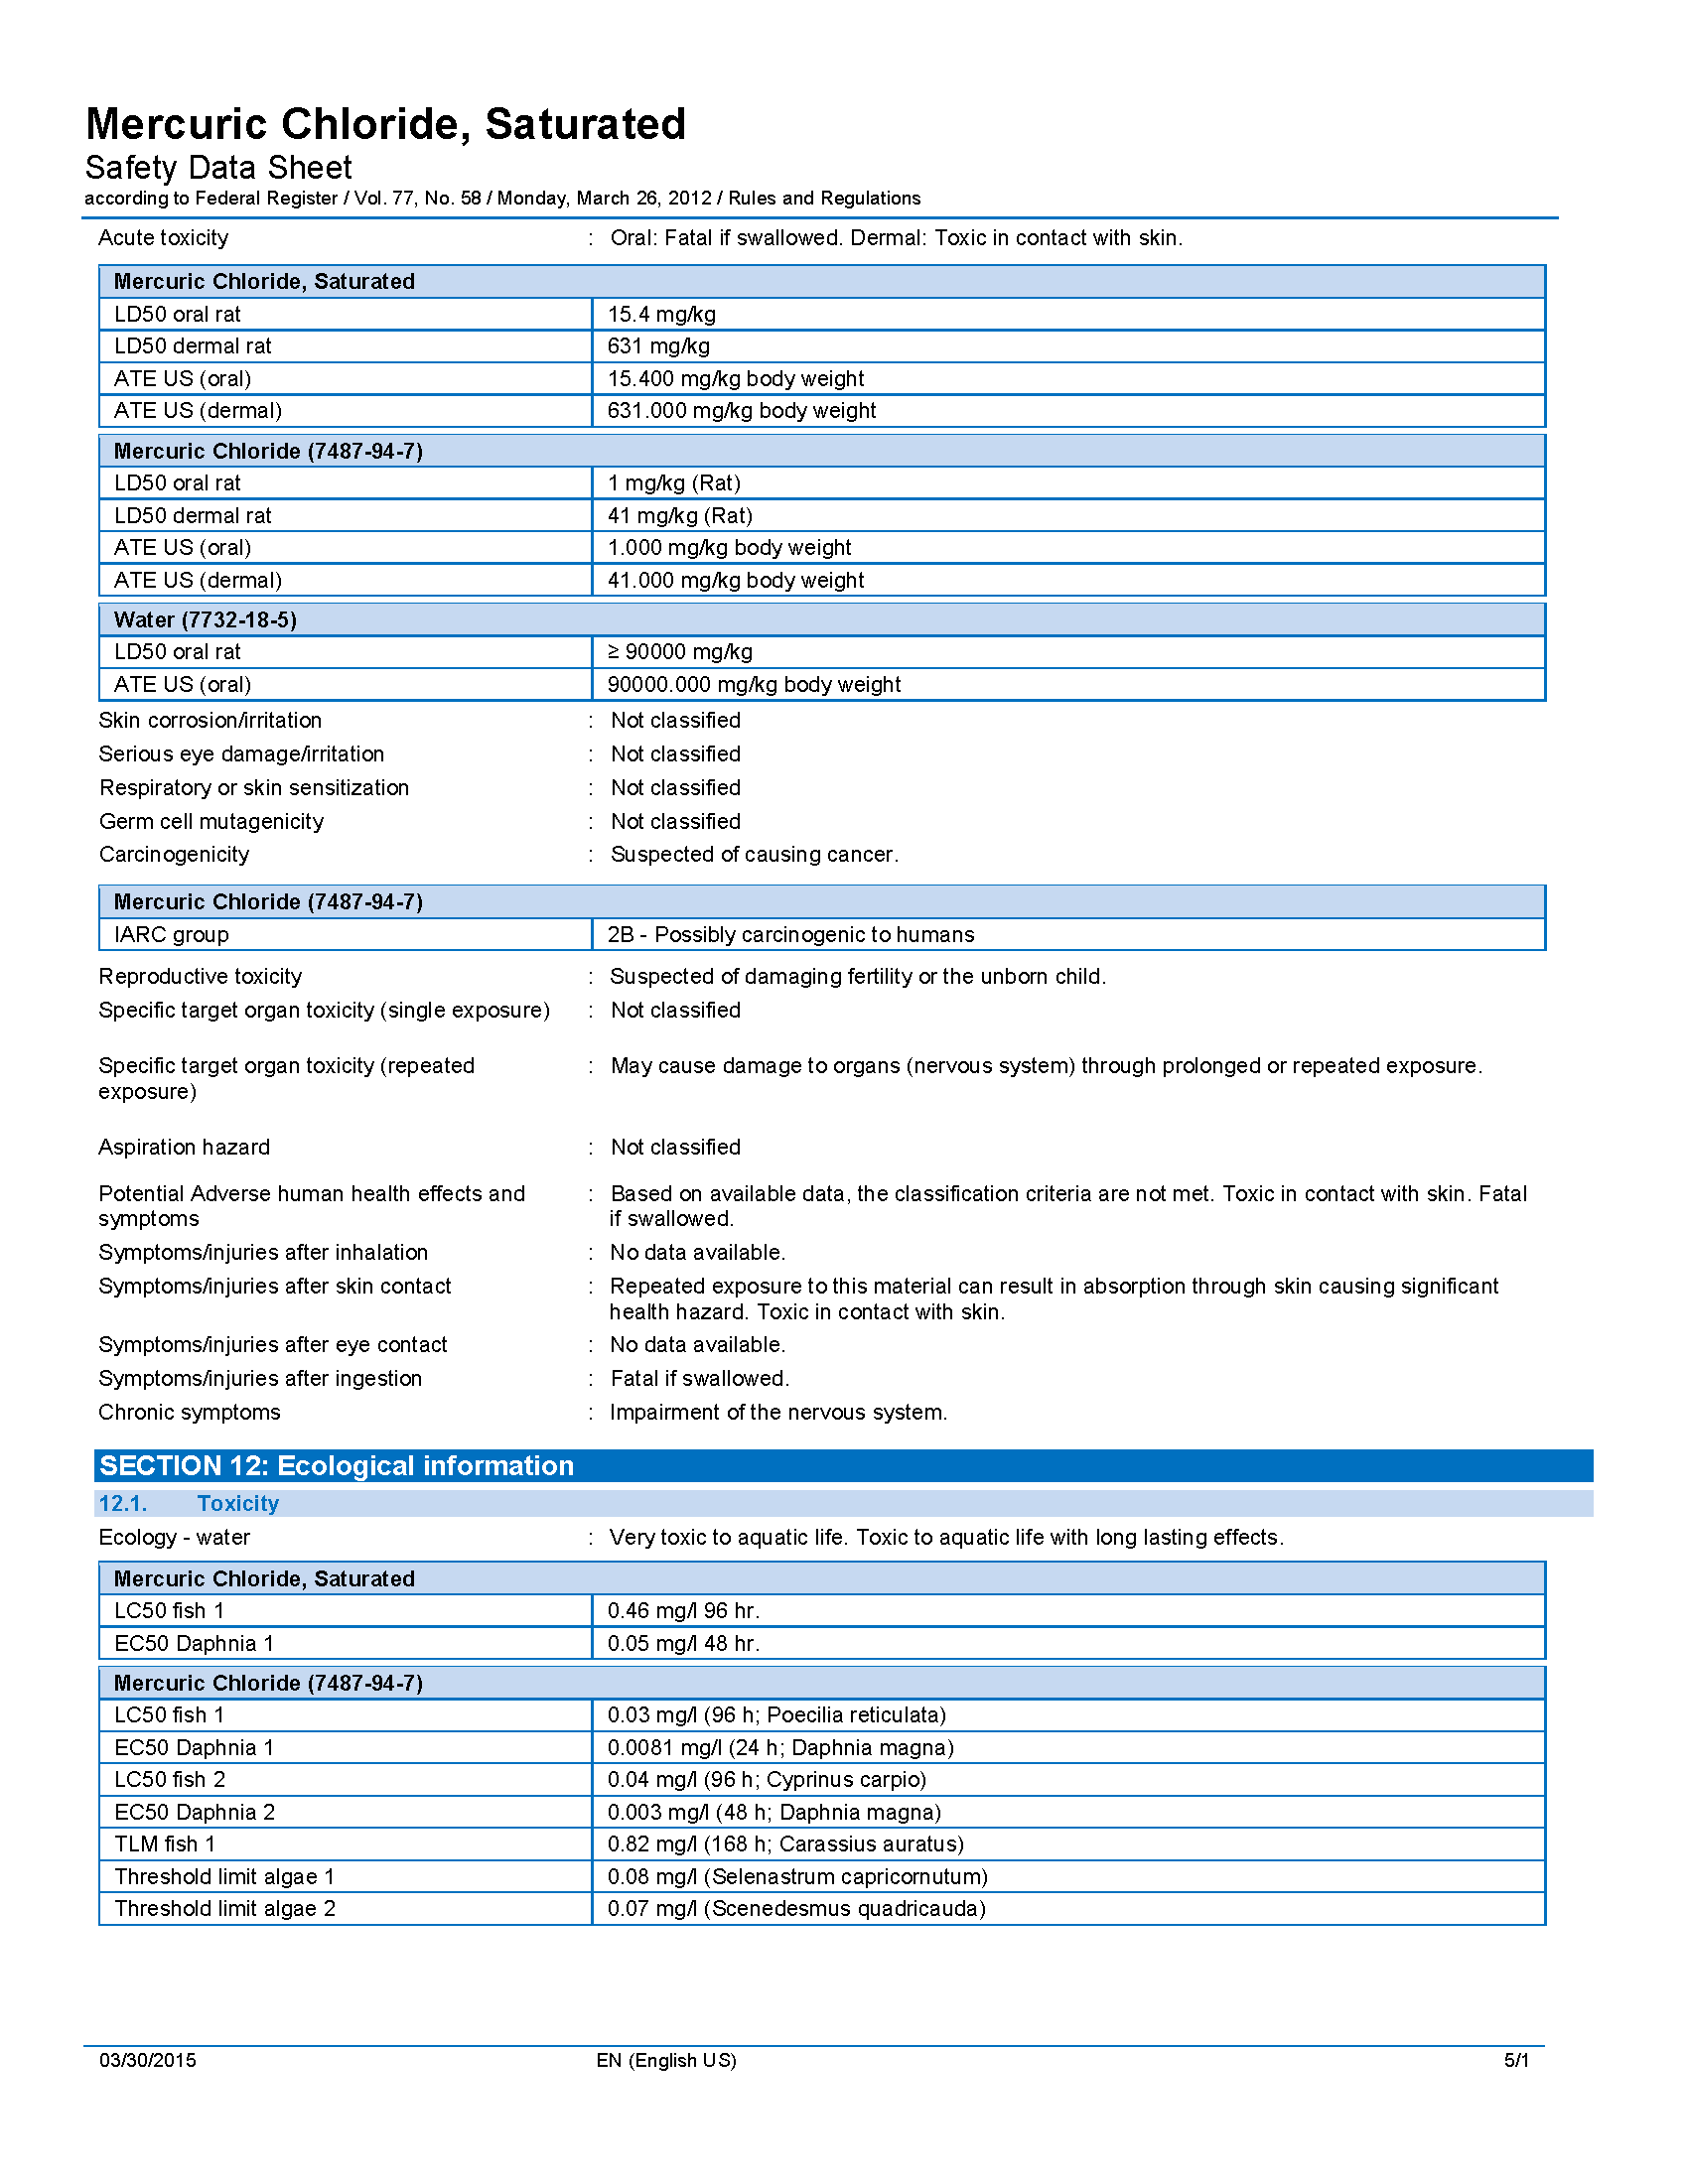
\includegraphics[width=1\textwidth,height=\textheight]{images/Saturated-Mercuric-Chloride-SDS_Page_5.png}
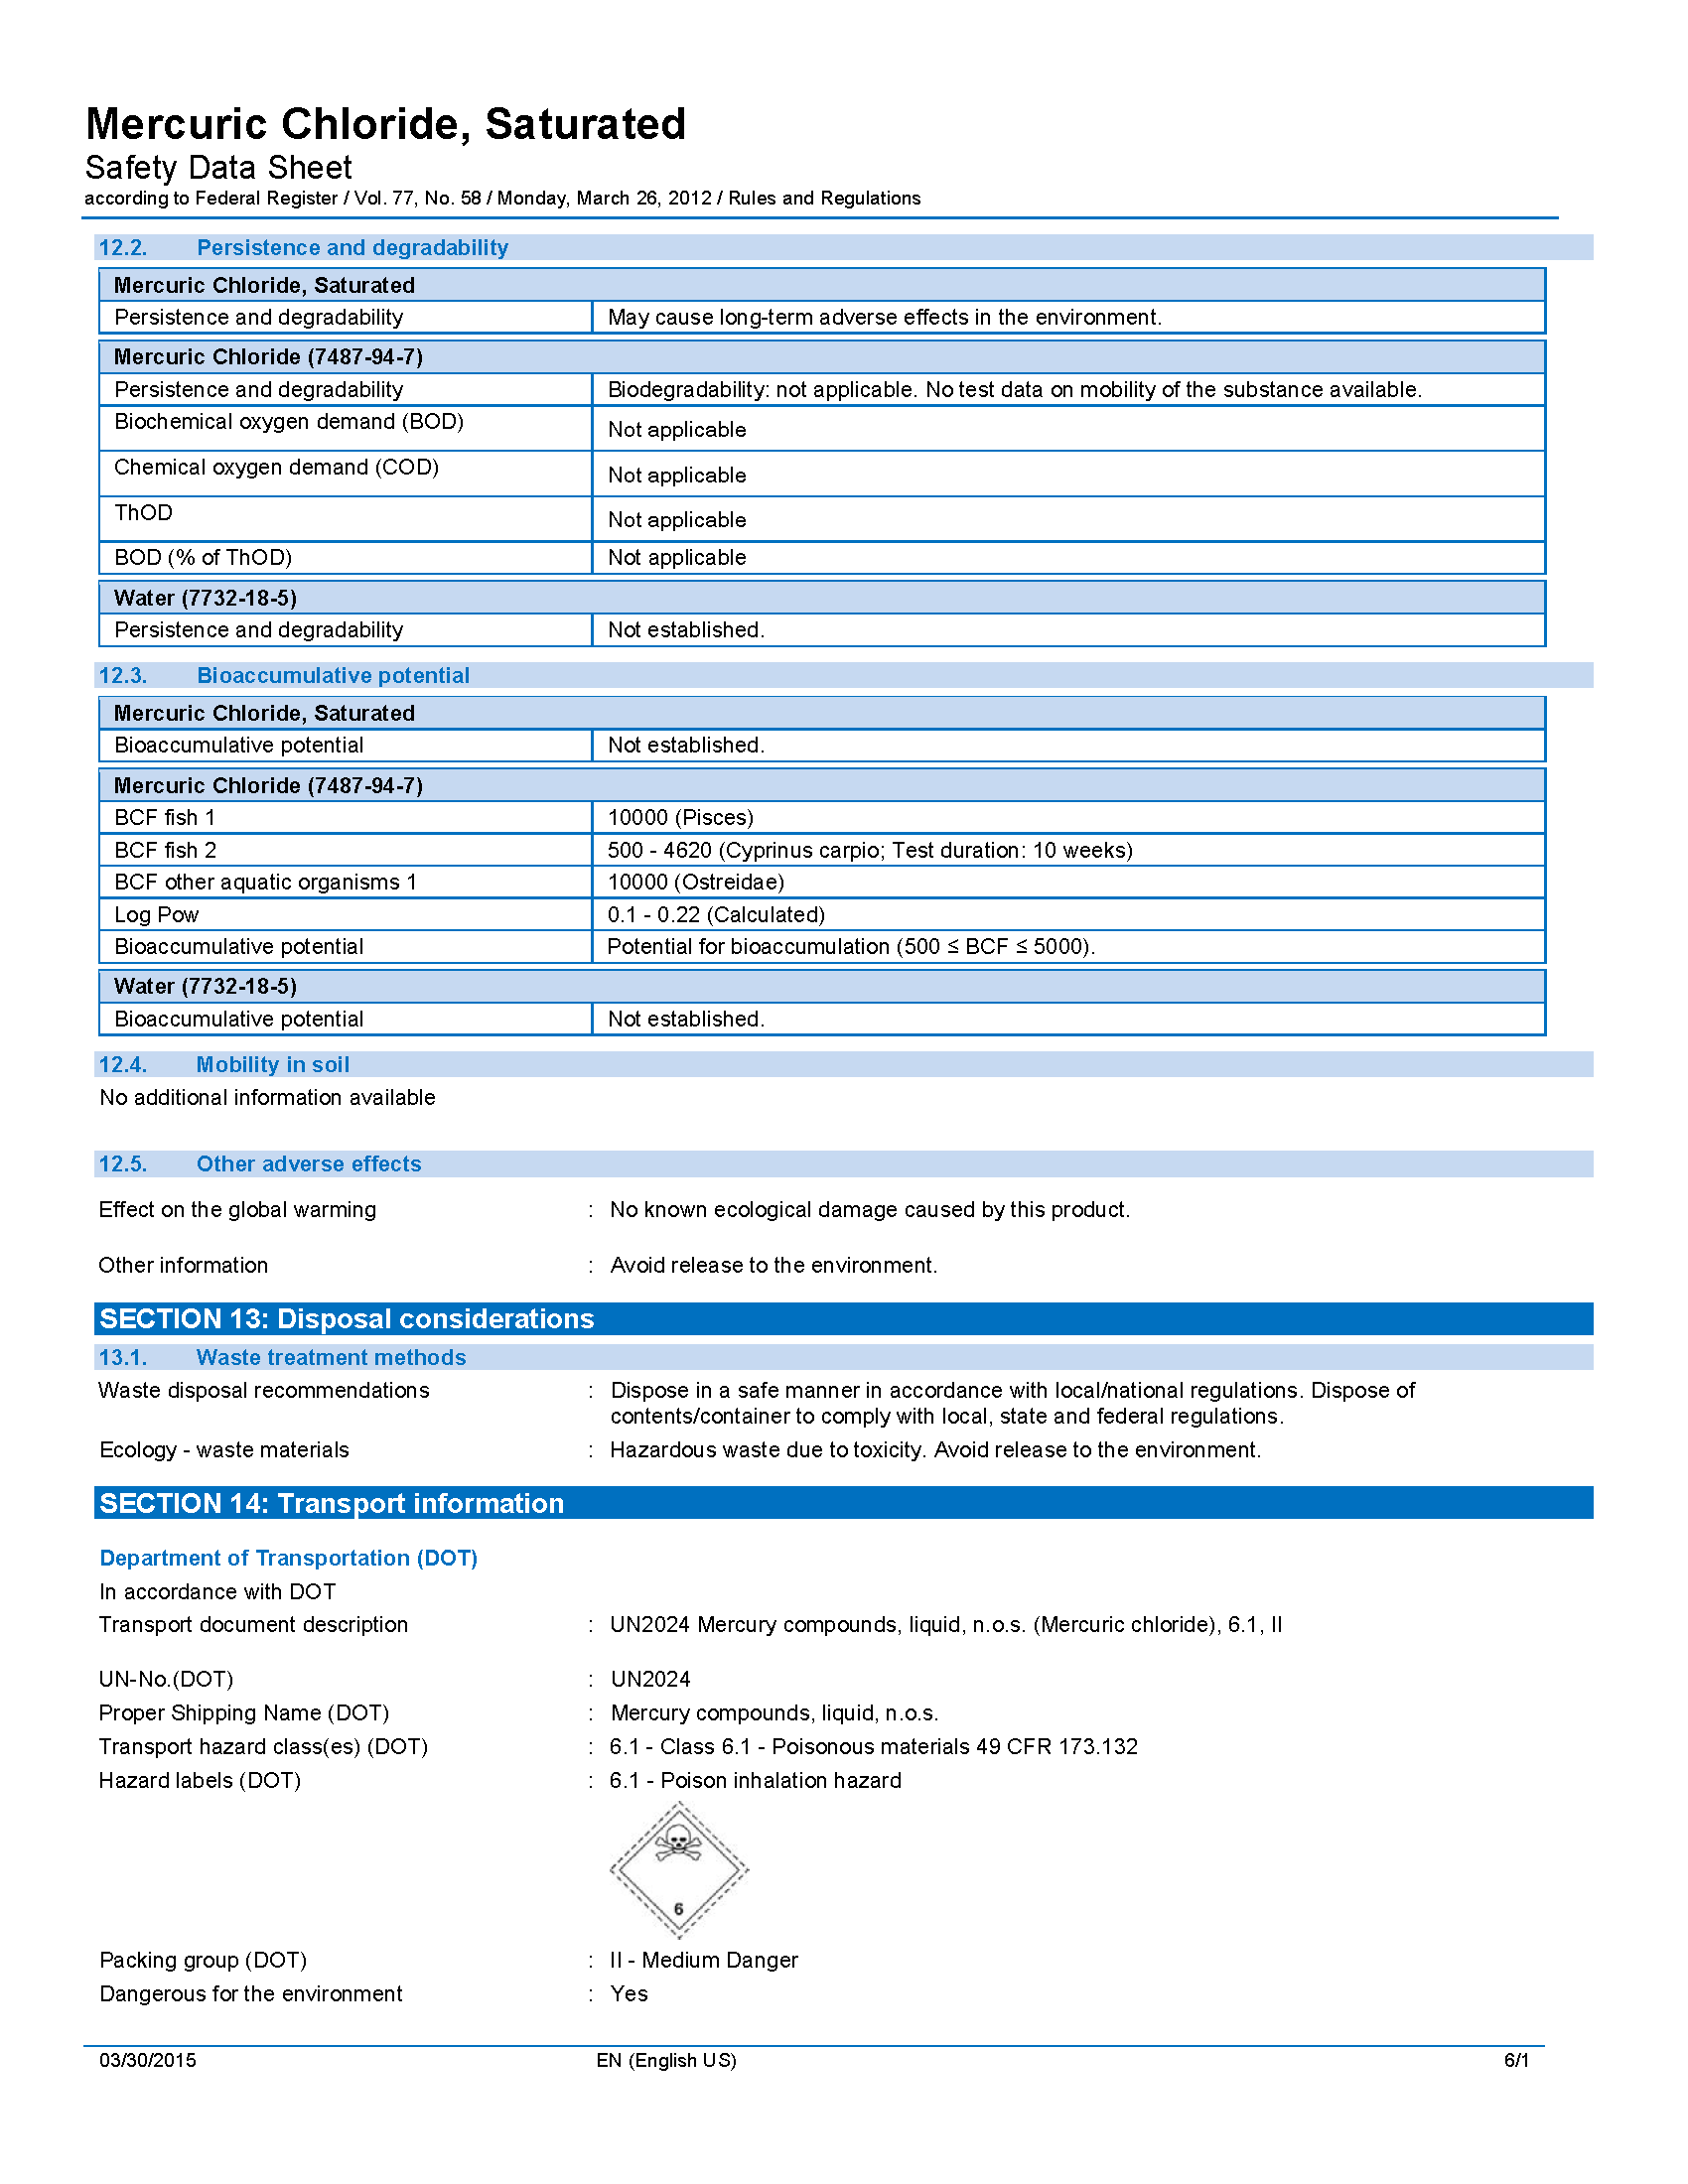
\includegraphics[width=1\textwidth,height=\textheight]{images/Saturated-Mercuric-Chloride-SDS_Page_6.png}
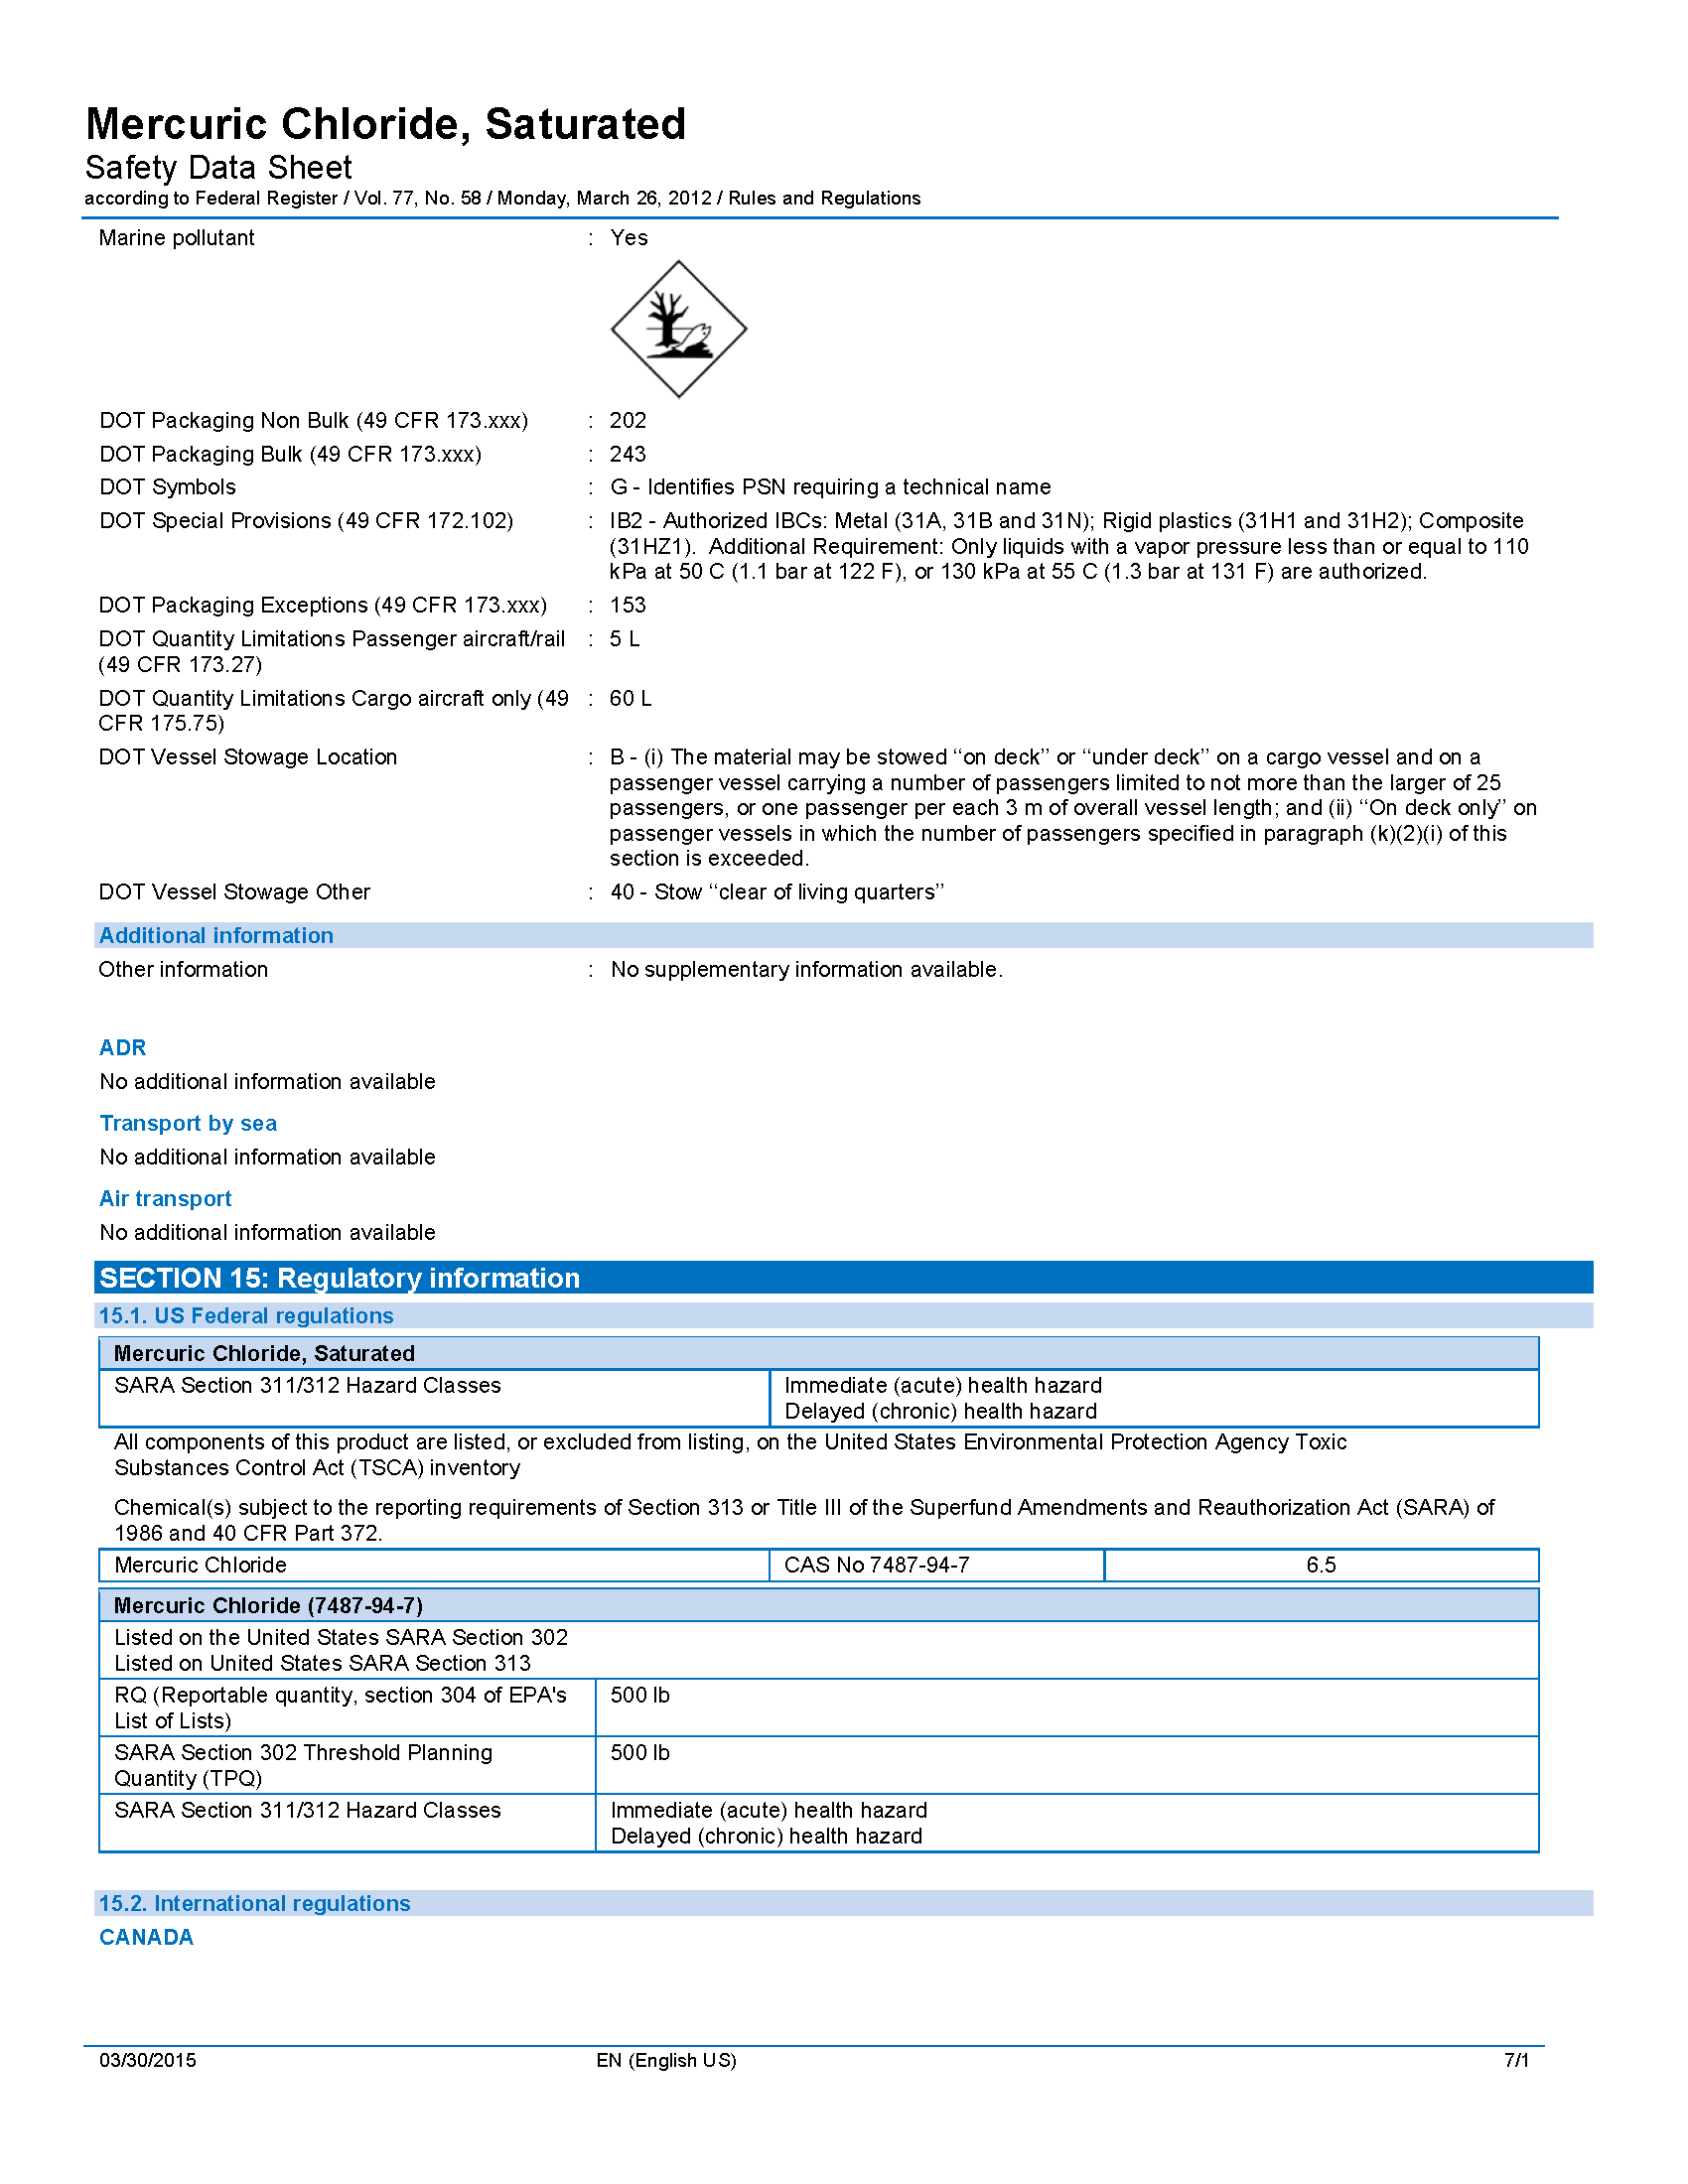
\includegraphics[width=1\textwidth,height=\textheight]{images/Saturated-Mercuric-Chloride-SDS_Page_7.png}
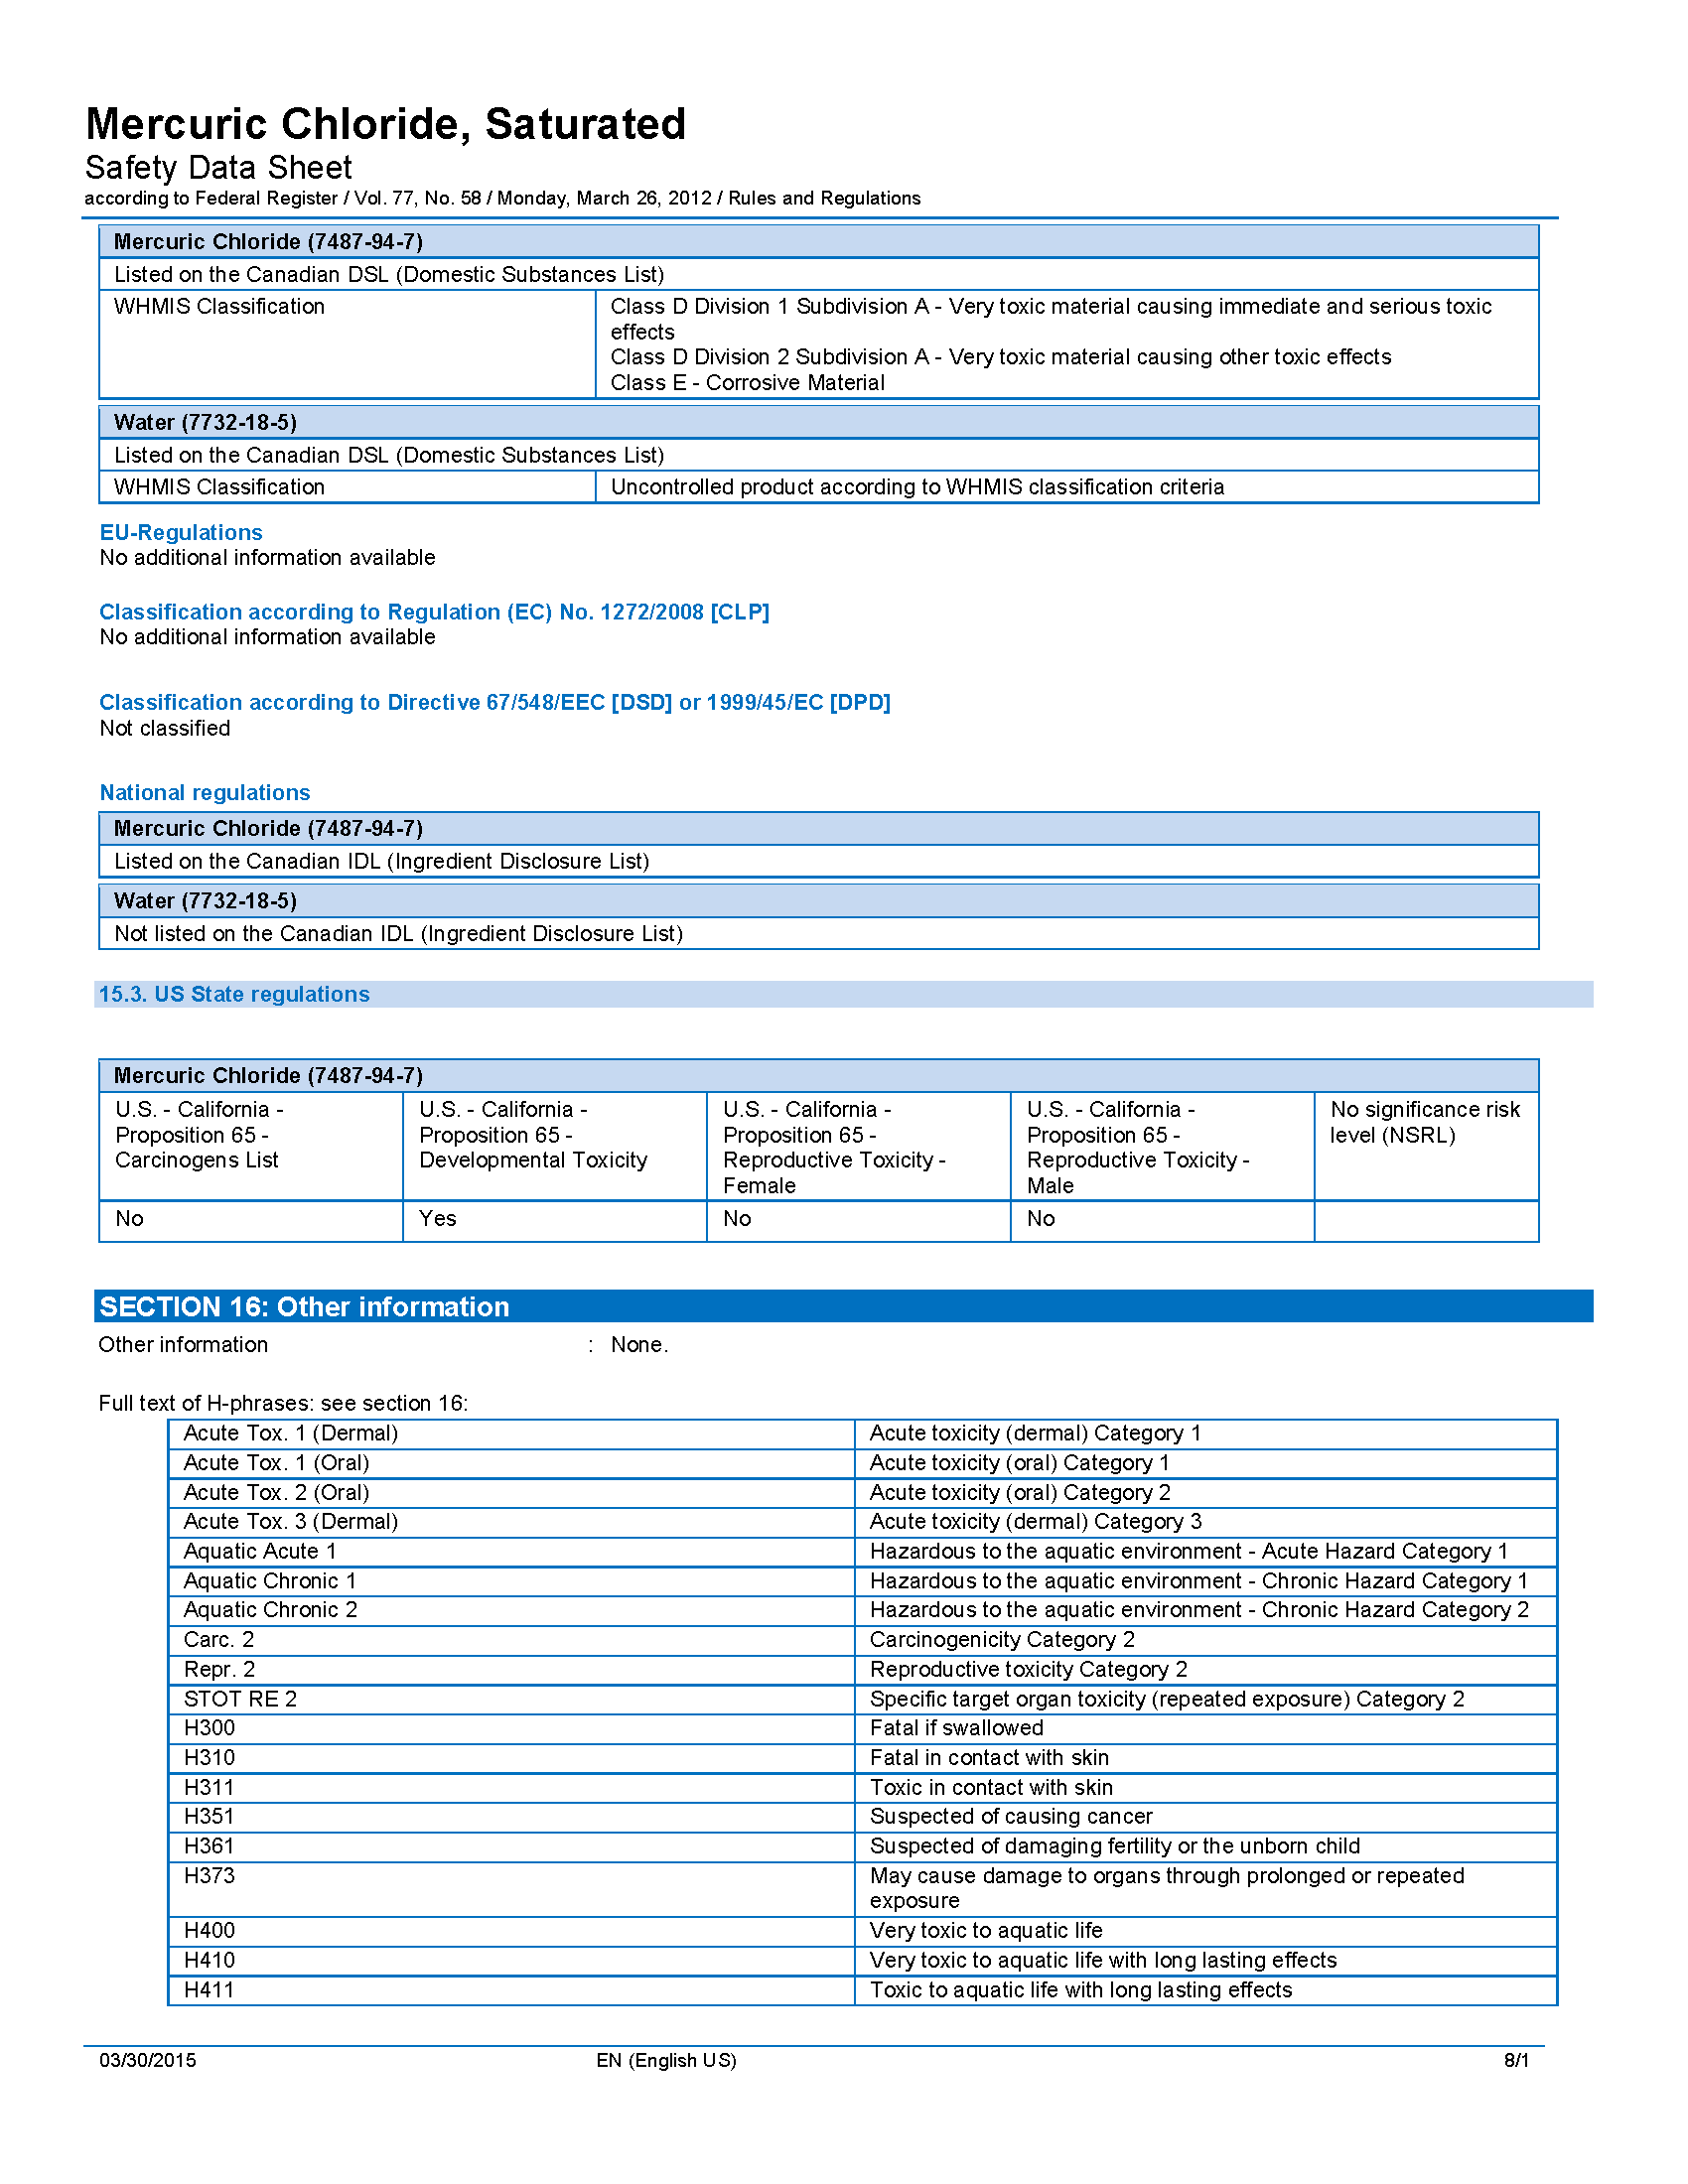
\includegraphics[width=1\textwidth,height=\textheight]{images/Saturated-Mercuric-Chloride-SDS_Page_8.png}
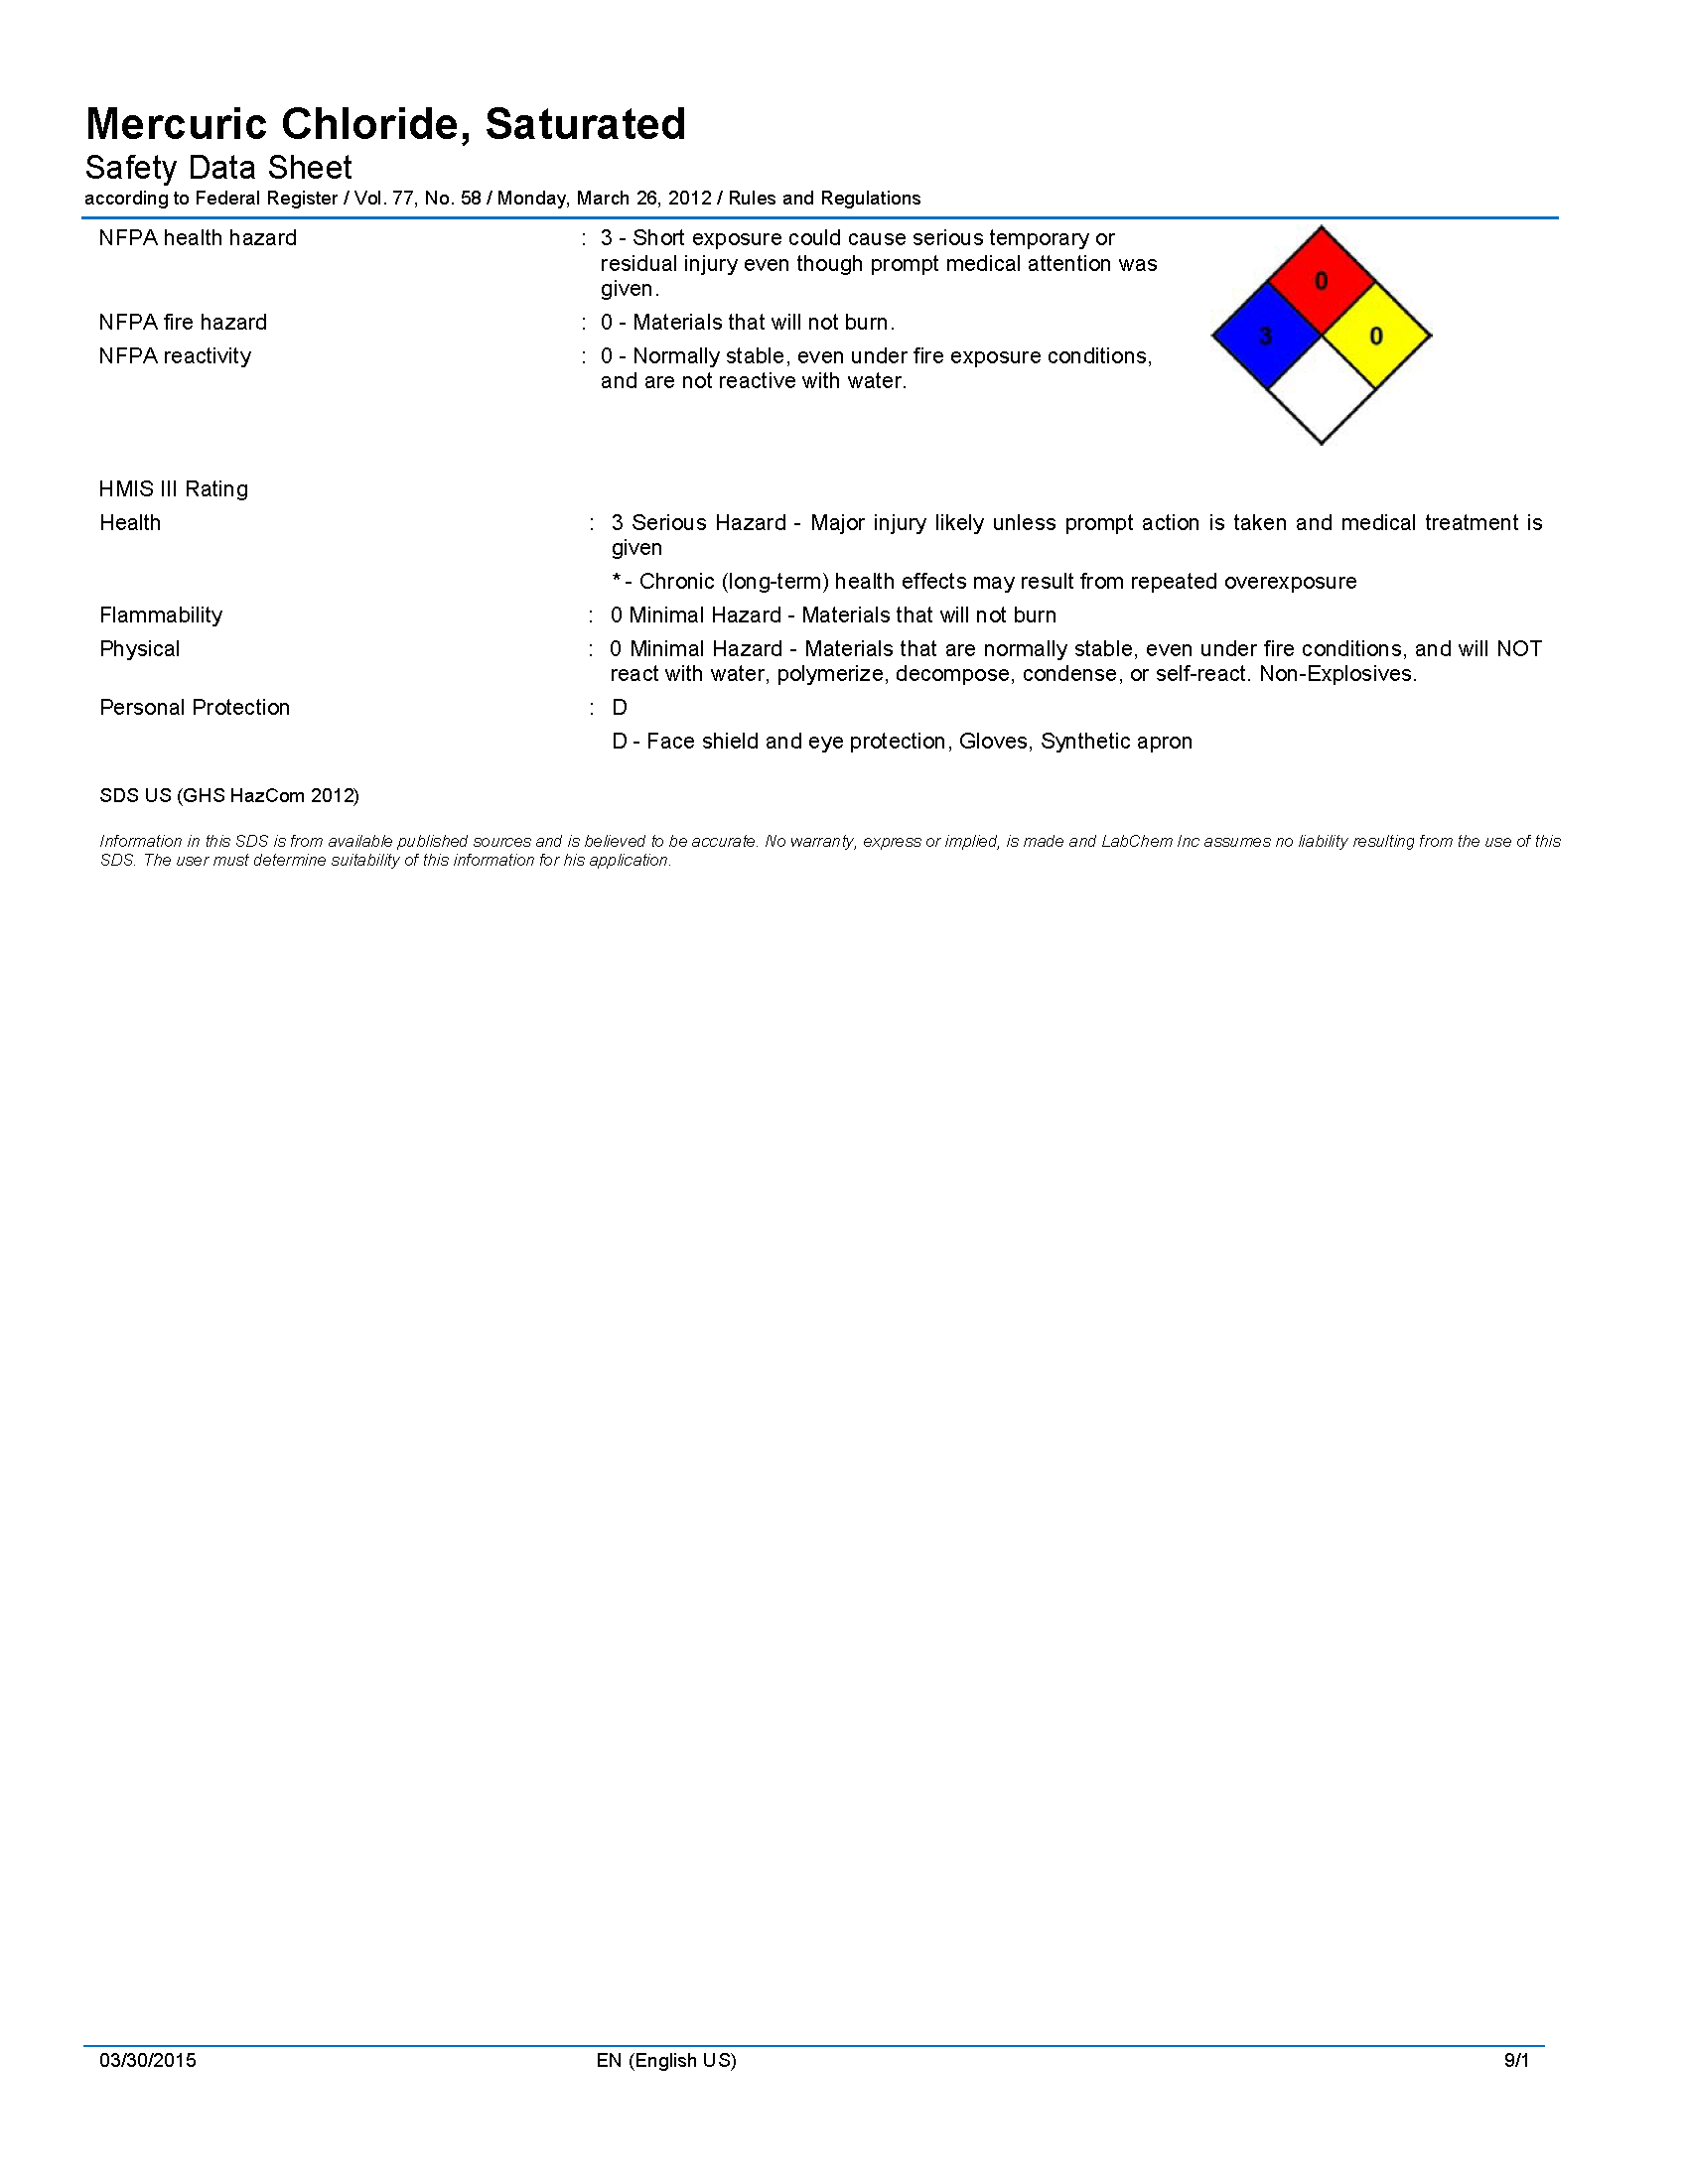
\includegraphics[width=1\textwidth,height=\textheight]{images/Saturated-Mercuric-Chloride-SDS_Page_9.png}
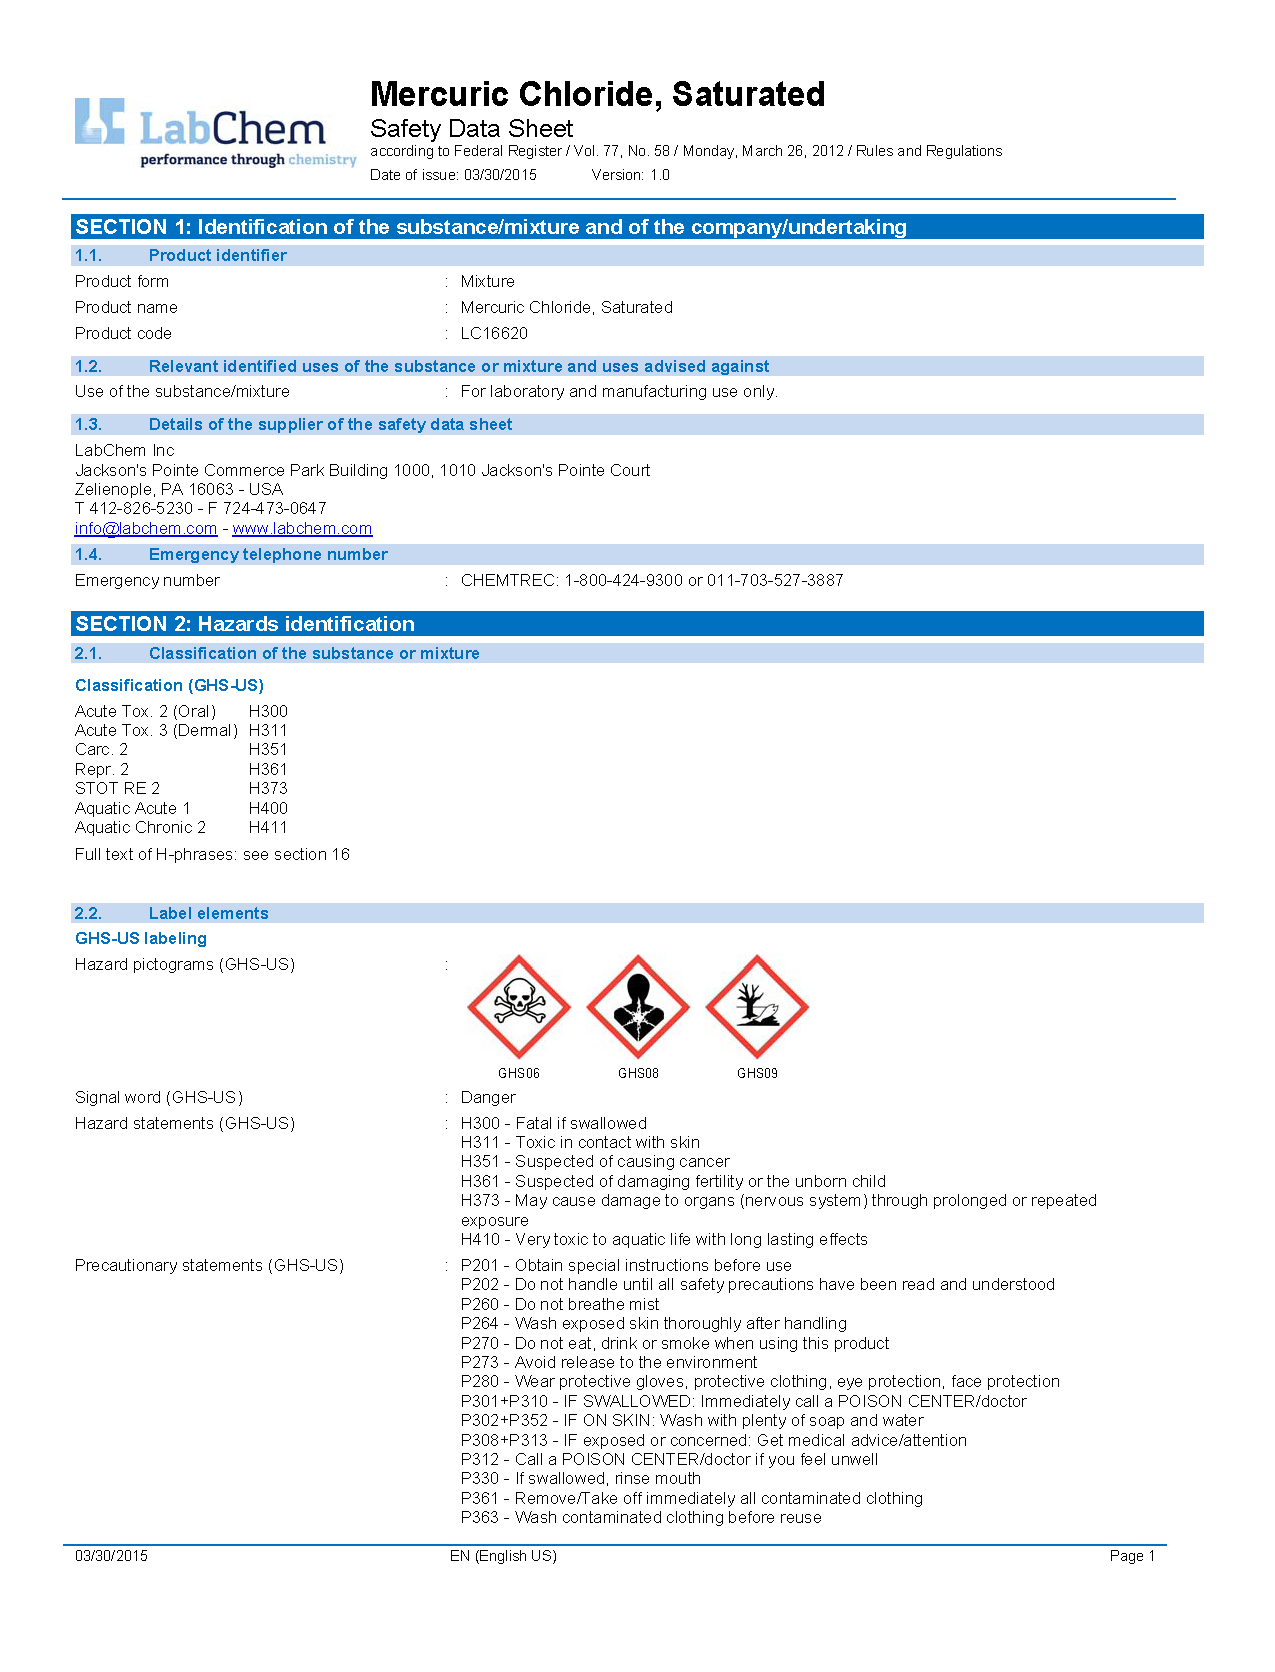
\includegraphics[width=1\textwidth,height=\textheight]{images/Saturated-Mercuric-Chloride-SDS_Page_1.png}

\hypertarget{data_processing}{%
\chapter{Data Processing and the Occ Package}\label{data_processing}}

The \emph{occ} package is uploaded to GitHub and can be downloaded directly in R.

\begin{enumerate}
\def\labelenumi{\arabic{enumi}.}
\tightlist
\item
  Open the \emph{devtools} library.
\end{enumerate}

\begin{Shaded}
\begin{Highlighting}[]
\KeywordTok{library}\NormalTok{(devtools)}
\end{Highlighting}
\end{Shaded}

\begin{enumerate}
\def\labelenumi{\arabic{enumi}.}
\setcounter{enumi}{1}
\tightlist
\item
  To download the \emph{occ} package, use the \texttt{install\_github} command. The repository name is in the form ``username/repo''. For the \emph{occ} package, the username is ``hannahbarkley'' and the repo is ``occ''. This install only need to occur once; however, the \emph{occ} package will need to be reinstalled if there are updates to the package (which is likely).
\end{enumerate}

\begin{Shaded}
\begin{Highlighting}[]
\KeywordTok{install_github}\NormalTok{(}\StringTok{"hannahbarkley/occ"}\NormalTok{)}
\end{Highlighting}
\end{Shaded}

\begin{enumerate}
\def\labelenumi{\arabic{enumi}.}
\setcounter{enumi}{2}
\tightlist
\item
  Once installed, load the \emph{occ} package.
\end{enumerate}

\begin{Shaded}
\begin{Highlighting}[]
\KeywordTok{library}\NormalTok{(occ)}
\end{Highlighting}
\end{Shaded}

\hypertarget{diel-suite}{%
\chapter{Diel Suite}\label{diel-suite}}

\hypertarget{diel-suite-underwater-checklist}{%
\section{Diel Suite Underwater Checklist}\label{diel-suite-underwater-checklist}}

PUC

\begin{enumerate}
\def\labelenumi{\arabic{enumi}.}
\tightlist
\item
  Tubes cleared of air and water with swipe of pump
\item
  Tubes connected to valves
\item
  Valves opened one full turn
\end{enumerate}

ADCP

\begin{enumerate}
\def\labelenumi{\arabic{enumi}.}
\tightlist
\item
  Ensure ADCP has unobstructed view of the surface
\item
  Get compass bearing on ADCP head direction after final installation
\end{enumerate}

\hypertarget{instruments}{%
\chapter{Instruments}\label{instruments}}

Guidance on instrumentation in the OMG is not intended to replace the instruction manual

\hypertarget{strs}{%
\section{STRs}\label{strs}}

All STRs must be programmed prior to deployment and have fresh batteries and dessicant installed. See manual's for specific programming guidance.

\textbf{STR - RBR Solo V3 Temperature Sensor}

Find the user manual in ``Reference'' section of OCC files at sea.

\textbf{Physical Preparation for Deployment}

\begin{itemize}
\item
  Use brand new Tadiran Lithium Thionyl Chloride 3.6v batteries
\item
  Wrap instrument housing with ``PVC floor marking tape'', leaving the serial number exposed
\end{itemize}

\textbf{Programming}

\begin{enumerate}
\def\labelenumi{\arabic{enumi}.}
\item
  Open Ruskin
\item
  Connect to the instrument with the supplies USB C cable, it should appear in the ``Navigator'' view after a few seconds
\item
  Ensure that your computer is connected to the internet so that the program can get the correct time from your computer.
\item
  Click UTC to set the instrument's time to UTC
\item
  Click on the ``Information'' tab and confirm that the battery has 3.6v
\item
  After programming each instrument, disconnect the USB cable, install a fresh desiccant and close the instrument in a short period of time so that the desiccant does not absorb ambient moisture in the air
\item
  Parameters
\end{enumerate}

\begin{enumerate}
\def\labelenumi{\alph{enumi}.}
\item
  Sampling Interval: 1 sample every 5 minutes
\item
  Sampling mode: Continuous
\end{enumerate}

\begin{itemize}
\item
  ``Ruskin\_instrument.log'' keeps a text file that includes the parameters of each instrument programmed
\item
  .rsk files are sqlight data files which are open source and non-proprietary
\end{itemize}

\textbf{Downloading Data from Solo 3}

\begin{enumerate}
\def\labelenumi{\arabic{enumi}.}
\item
  Connect to the instrument
\item
  Select the dataset and download it
\end{enumerate}

\textbf{Processing RBR Solo 3 Data Files}

see \protect\hyperlink{data_processing}{Data Processing with the OCC Package}

\textbf{Factory Recalibration of the Solo 3}

\begin{itemize}
\item
  Call RBR to arrange the re-calibration of each Solo 3, which will cost approx. \$120
\item
  Instrument drift over 3 years should be less than .006 C, thus there is no need to re-calibrate the data set with post-cruise calibration coefficients
\item
  In Ruskin, by default, the name of a data file is composed of the following information:

  \begin{itemize}
  \tightlist
  \item
    The first six digits represent the logger serial number.
  \item
    The next eight digits represent the current year, month, and day.
  \item
    The next four digits represent the current time to the minute.
  \item
    The file extension indicates the file format and should not be changed. If you change it, the file extension that you specify becomes part of the name, and the required extension is appended. For example, the file named 911936\_20090522\_1613.rsk contains data for a logger with a serial number of 911936 whose data was downloaded in 2009 on May 22 at 4:13 pm.
  \end{itemize}
\end{itemize}

\hypertarget{fc}{%
\chapter{Field Checklists}\label{fc}}

\hypertarget{daily-tasks-for-the-team}{%
\section{Daily Tasks for the Team}\label{daily-tasks-for-the-team}}

\href{https://drive.google.com/open?id=1I4Hojo0qjKtUwhRqgc9aLM6_fGtjqZMM}{Find Excel version here via Google Drive}

\textbf{STR}

\begin{itemize}
\tightlist
\item
  Before Ops

  \begin{itemize}
  \tightlist
  \item
    assemble, program and stage needed STRs
  \item
    confirm 10 36'' cable ties for each STR planned
  \item
    write serial numbers of planned STR deployments on tomorrow's data sheet
  \end{itemize}
\item
  After Ops

  \begin{itemize}
  \tightlist
  \item
    download strs
  \item
    enter deployments and retreivals into mooring database
  \item
    import waypoints into mooring database
  \item
    clean STRs, put weights and brackets on fantail or in DD bath
  \end{itemize}
\end{itemize}

\textbf{CAU}

\begin{itemize}
\tightlist
\item
  Before Ops

  \begin{itemize}
  \tightlist
  \item
    Pack supplies for planned CAU site swaps
  \item
    write down deploy CAU SNs on tomorrow's data sheet
  \end{itemize}
\item
  After Ops

  \begin{itemize}
  \tightlist
  \item
    scrape/record CAU SN's, re-bag and freeze with cruise \& site label
  \item
    dispose of old clips and stakes
  \item
    after CTD/H2O data is entered, give data sheets to data manager
  \end{itemize}
\end{itemize}

\textbf{Water Sampling and CTD}

\begin{itemize}
\tightlist
\item
  Before Ops

  \begin{itemize}
  \tightlist
  \item
    DIC bottles and all supplies in each kit
  \item
    Niskin, line, messenger, weight staged for each CTD
  \end{itemize}
\item
  After Ops

  \begin{itemize}
  \tightlist
  \item
    rinse and stage CTDs
  \item
    Swap full bottles for empties, dispose of waste
  \item
    restock all supplies
  \item
    replace and label any worn ziplocs
  \item
    enter CTD and water sample log into CTD/H2O Database (hopefully this is not a necessary step on MARAMP 2020!)
  \end{itemize}
\end{itemize}

\textbf{GPS Units (for OCC and benthic/fish GPS)}

\begin{itemize}
\tightlist
\item
  Drop off GPS units with data manager for waypoiont download
\end{itemize}

\textbf{Cameras}

\begin{itemize}
\tightlist
\item
  Before Ops

  \begin{itemize}
  \tightlist
  \item
    Ensure cameras are set to UTC time
  \item
    Ensure cameras have memory cards
  \item
    charge camera batteries
  \item
    clean camera housings
  \item
    bake desiccants and install them
  \end{itemize}
\item
  After Ops

  \begin{itemize}
  \tightlist
  \item
    download and sort photos
  \item
    download and sort photoquad photos
  \item
    charge cameras or swap charged batts for used batts
  \item
    install new dessicants
  \end{itemize}
\end{itemize}

\textbf{Stage all Gear}

\begin{itemize}
\tightlist
\item
  Action packer packed for day of ops
\item
  Pam float and reel staged
\item
  If deep STR: Marker Float and drop weight
\item
  1 full bag of large cable ties (keep on boat)
\item
  CTDs and lines
\end{itemize}

\textbf{Other}

\begin{itemize}
\tightlist
\item
  gauge tanks
\end{itemize}

\hypertarget{where-to-save-data}{%
\section{Where to Save Data}\label{where-to-save-data}}

\href{https://drive.google.com/open?id=16l1OQgGEunLoADh_MEGyIfbQL2w0u6aw}{Checkout this Excel file on Google Drive for details on where to save data}


\end{document}
